\documentclass[12pt,a4paper,openany]{book}
\usepackage{amssymb, amsmath}
% \usepackage[polish]{babel}
\usepackage[utf8]{inputenc}
\usepackage[T1]{fontenc}
\usepackage[dvips]{graphicx}
\setlength{\parindent}{7mm}
\setlength{\parskip}{4mm}
\usepackage{indentfirst}
\usepackage{mathtools}
\usepackage{enumitem}
\usepackage{titlesec}
\usepackage{paralist}
\usepackage{comment}
\usepackage{bigints}
\usepackage{hyperref} 
\usepackage{accents}
\usepackage{amsthm}
\usepackage{graphicx}
\usepackage{amsmath}
\usepackage{float}
\restylefloat{table}
\usepackage{bm}
\usepackage[table,xcdraw]{xcolor}
\usepackage{pdfpages}
%\usepackage{subfig}
\usepackage{subcaption}
\usepackage{lipsum}

\titleformat{\chapter}[display]
  {\normalfont\bfseries}{}{0pt}{\Large}


\usepackage{xpatch}
\makeatletter
\xpatchcmd{\@thm}{\thm@headpunct{.}}{\thm@headpunct{}}{}{}
\makeatother

\graphicspath{ {figs/} }

\newtheorem{definition}{Definition}


\newcommand{\ubar}[1]{\underaccent{\bar}{#1}}
  \let\itemize\compactitem
  \let\enditemize\endcompactitem
  \let\enumerate\compactenum
  \let\endenumerate\endcompactenum
  \let\description\compactdesc
  \let\enddescription\endcompactdesc
  \pltopsep=1pt
  \plitemsep=1pt
  \plparsep=1pt

\newcommand\myeq{\mathrel{\overset{\makebox[0pt]{\mbox{\normalfont\tiny\sffamily $\lambda > 0$}}}{=}}}

\titleformat{\chapter}[display]   
{\normalfont\huge\bfseries}{\chaptertitlename\ \thechapter}{20pt}{\Huge}   
\titlespacing*{\chapter}{0pt}{-10pt}{40pt}

\titlespacing*{\section}{0pt}{1.\baselineskip}{\baselineskip}


\linespread{1.4}

\pagestyle{myheadings}
\pagestyle{plain}
\usepackage{geometry}
\newgeometry{tmargin=2.5cm, bmargin=2.5cm, lmargin=3cm, rmargin=2.5cm}
\newcommand\setItemnumber[1]{\setcounter{enumi}{\numexpr#1-1\relax}}
\newcommand*{\QEDB}{\hfill\ensuremath{\square}}
\newcommand{\ignore}[1]{}

\newcommand{\RomanNumeralCaps}[1]
    {\MakeUppercase{\romannumeral #1}}

\begin{document}

\begin{titlepage}
\begin{flushleft}
\end{flushleft}
\begin{center}
\textsc{{\huge Politechnika Warszawska}}
\end{center}
\bigskip
\bigskip
\begin{center}
\textsc{{\Large Wydział ...}}
\end{center}
\bigskip
\bigskip
\begin{center}
\begin{Large}
Kierunek: ...
\end{Large}
\end{center}
\bigskip
\bigskip
\noindent\hrulefill
\begin{center}
\textsc{\textbf{{\large ...
\\}}}
\bigskip
\bigskip

{\large 
Adam Komorowski i Maciej Domagała}

\end{center}
\noindent\hrulefill
\bigskip
\bigskip
\begin{center}
\end{center}
\bigskip
\bigskip
\bigskip
\bigskip
\begin{center}
{\textsc{\large Warszawa, czerwiec 2021
}}
\end{center}
\end{titlepage}

\tableofcontents

\chapter*{Introduction}
\addcontentsline{toc}{chapter}{Introduction}

\noindent As of now, we can describe the developments and current state of the matter in the CLIP related modeling as highly experimental and creative. Given the subjective nature of GAN models, need for empirical validation of results and lack of all-round metrics for proper evaluation, there are currently no useful methods of comparing different approaches. We try to address this issue by performing evaluation on different classifiers and datasets. We also show that it is possible to use the latent space search methods research previously and combine them with CLIP model. 

\chapter{Theory}

\section{Generative Adversarial Networks}

%https://machinelearningmastery.com/what-are-generative-adversarial-networks-gans/
%https://jonathan-hui.medium.com/gan-whats-generative-adversarial-networks-and-its-application-f39ed278ef09
%https://jonathan-hui.medium.com/gan-some-cool-applications-of-gans-4c9ecca35900
%https://realpython.com/generative-adversarial-networks/
%https://machinelearningmastery.com/how-to-code-the-generative-adversarial-network-training-algorithm-and-loss-functions/
%https://arxiv.org/pdf/1406.2661.pdf

\subsection{Overview}

\noindent Generative Adversarial Networks (GANs) is a family of neural networks used in generative modelling. They were proposed in 2014 by Ian Goodfellow et al. in \cite{gan}.\\
\noindent They have various different applications across deep learning fields e.g. generative models can be used as a tool for data augmentation of small datasets. For instance, one can feed some text written in a particular handwriting as input to a generative model to generate more text in the same handwriting. The following are results of the first facial images generation experiments with GANs. Another use case is generation of super-resolution images, which allows to produce more detailed and high quality version of input images. 
 \begin{figure}[ht!]
     \centering
     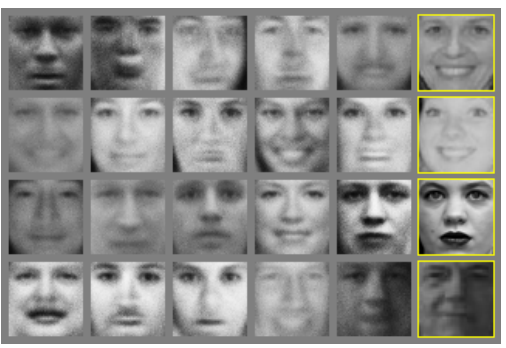
\includegraphics[scale=0.4]{figs/faces.png}
     \caption{Images generated by GAN \cite{gan}.}
 \end{figure}
 \newpage
\noindent Since first examples, GANs networks became an object of intense development, which resulted in increasing quality of generated objects each year.
 \begin{figure}[ht!]
     \centering
     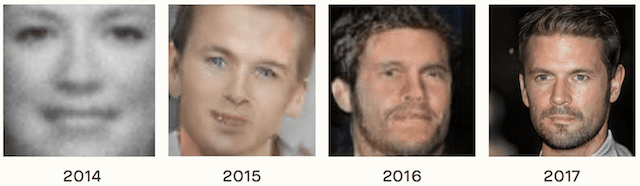
\includegraphics[scale=0.5]{figs/gan_progression.png}
     \caption{Example of progression in the capabilities of GANs \cite{ganprogress}. }
 \end{figure}
 \newline
%In our work, we will describe the architectures of two state of the art GAN models, StyleGAN and BigGAN.
\subsection{Architecture}
\noindent Generative adversarial networks are composed of two neural networks, one called the \textbf{generator} (denoted as G in this work) and the other called the \textbf{discriminator} (denoted as D). \\
\noindent The role of the generator is to estimate the probability distribution of the real samples in order to provide generated samples resembling real data. The discriminator is trained to estimate the probability that a given sample came from the real data rather than being provided by the generator.
\noindent These structures are called generative adversarial networks because the generator and discriminator are trained to compete with each other: the generator tries to get better at fooling the discriminator, while the discriminator tries to get better at identifying generated samples.  GAN architecture can be described using schema below.
 \begin{figure}[H]
     \centering
     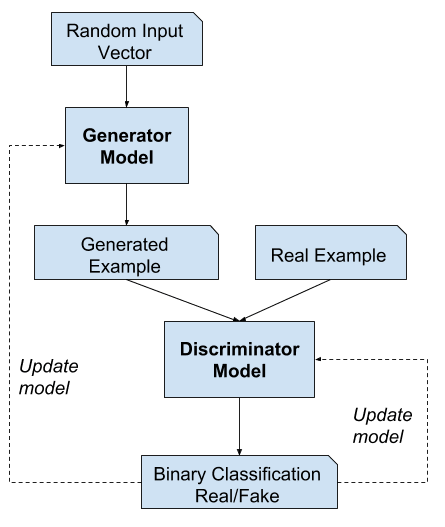
\includegraphics[scale=0.3]{figs/gan_architecture.png}
     \caption{GAN architecture.}
 \end{figure}

\subsubsection{Training}
\noindent The GAN training process consists of a two-player minimax game.  Although the dataset containing the real data isn’t labeled, the training processes for discriminator and generator are performed in a supervised way.  \\
\noindent For discriminator training, at each iteration we pass some real samples taken from the training data labeled as $1$ and some generated samples provided by generator labeled as $0$. New images are generated based on noise input derived from e.g. Gaussian distribution. This way, we can use more conventional supervised training frameworks to update the parameters of discriminator. The discriminator outputs a value $D(x)$ indicating the chance that x is a real image. Model objective is to maximize the chance of recognizing real images and generated images as separate classes. To measure the performance the \textbf{cross-entropy loss} is used and therefore the objective function can be written as follows:

\begin{equation}
max_{D} V(D) = \mathbb{E}_{\textbf{x} \sim p_{data}(\textbf{x})} [\log D(\textbf{x})] + \mathbb{E}_{\textbf{z} \sim p_{z}(\textbf{z})} [\log(1-D(G(\textbf{z})))].
\end{equation}

\noindent For each batch of training data containing labeled real and generated samples, model updates the parameters of discriminator to optimize the loss function. After the parameters are updated, generator is trained to produce better samples (in terms of quality and variety). The output of generator is connected to discriminator, whose parameters are kept frozen at the time of generator training. On the generator side, it's objective is to generate images with the highest possible value of $D(x)$ to \textit{fool} the discriminator. This condition can be written as:

\begin{equation}
min_{G} V(G) = \mathbb{E}_{\textbf{z} \sim p_{z}(\textbf{z})} [\log(1-D(G(\textbf{z})))].
\end{equation}

\noindent Combining these two aspects, we can define GAN as a minimax game during which generator wants to minimize V function, while discriminator wants to maximize it:

\begin{equation}
min_{G} max_{D} V(D, G) =  \mathbb{E}_{\textbf{x} \sim p_{data}(\textbf{x})} [\log D(\textbf{x})] + \mathbb{E}_{\textbf{z} \sim p_{z}(\textbf{z})} [\log(1-D(G(\textbf{z})))].
\end{equation}

\noindent Once both objective functions are defined, they are learned jointly by the alternating gradient descent. We fix the generator model’s parameters and perform a single iteration of gradient descent on the discriminator using the real and the generated images. Then the roles are switching and the discriminator is fixed while the generator is trained for another single iteration. We train both networks in alternating steps until the generator produces good quality images. The training algorithm for GANs is well summarized in the figure below.

 \begin{figure}[ht!]
     \centering
     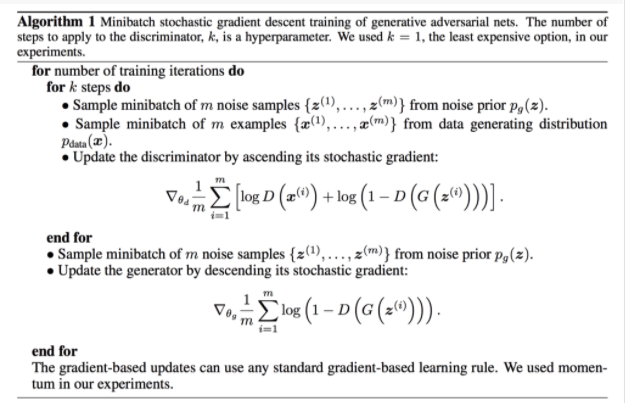
\includegraphics[scale=0.7]{figs/gan_algo.png}
     \caption{GAN training algorithm pseudocode \cite{gan}.}
 \end{figure}
 
\noindent It is worth mentioning that a known problem of GAN networks is the fact that not always a smaller value of loss function leads to better results - in practice, a common solution is to empirically evaluate generated results every few iterations, rather than tracking loss. To cope with this problem metrics such as \textbf{Inception Score} or \textbf{Frechet Inception Distance} were presented. 
%These will be described in detail in the following sections.

\subsubsection*{Inception Score and Fr\'echet Inception Distance}

%https://www.coursera.org/lecture/build-better-generative-adversarial-networks-gans/inception-score-HxtYM
%https://medium.com/octavian-ai/a-simple-explanation-of-the-inception-score-372dff6a8c7a
%https://arxiv.org/pdf/1606.03498.pdf
%https://arxiv.org/pdf/1801.01973.pdf - good one, maybe use.


\noindent \textbf{Inception Score} is a metric used especially for measuring the quality of Generative Adversarial Network outputs. It was first proposed in \cite{improvedgans} and was used ever since to compare benchmark results of new generative models. Inception Score was defined to measure two important aspects of generative networks performance - quality of generated images and their diversity. If network produces diverse images of good quality - the score is designed to be high.\

%Usually, objective function used in generative-discriminator type of network is representing how well one part of the architecture is performing in comparison to the other part e.g. how well discriminator is detecting generated images. This does not provide a measurable information about the quality and diversity of images though.\

\noindent Authors used the Inception network \cite{inception} to calculate the conditional label distribution for every created image. It is denoted as $p(y|x)$, where y is bounded to label and $x$ is a single image instance. For images of high quality this distribution should have a \textit{low entropy} characteristic - meaning that one class (correct one) should have a high probability score, while the rest should have relatively small scores. This indicates that Inception classifier has a lot of certainty what is presented on given image.\ 
To measure diversity, authors proposed to calculate the marginal distribution of $y$ by combining label distributions for a large set of images (50 000 is a proposed value). More formally, if $z$ is a latent vector and $G(z)$ is an image generated from the vector, then marginal distribution 

\begin{equation}
p(y) = \int_{z} p(y \mid x=G(z)) \phantom{v} dz
\end{equation}

\noindent should have \textit{high entropy} (should be close to the uniform distribution) if model has a strong diversifying power.\

\noindent Combining two above conditions, we can observe that best performing model would have different distributions of $p(y|x)$ and $p(y)$. To link these two discrete distributions together authors decided to use a Kullback-Leibler Divergence formula:

\begin{equation}
D_{K L}(p \| q)=\sum_{i=1}^{N} p\left(x_{i}\right) \cdot\left(\log p\left(x_{i}\right)-\log q\left(x_{i}\right)\right),
\end{equation}

\noindent where $p$ and $q$ are two distributions for which we want to calculate relative entropy. Combining this formula with exponent (for easier comparison between different results) we obtain final Inception Score definition:

\begin{equation}
\operatorname{IS}(G)=\exp \left(\mathbb{E}_{\mathbf{x}} D_{K L}(p(y|x) \| p(y))\right)
\end{equation}

%\noindent Inception Score has several limitations (pointed out in \cite{noteonis}):
%
%\begin{itemize}
%\item Scoring is irreversibly bounded to Inception model and its training data. There could be low IS scoring for generating objects not in primary training data or using labels not incorporated by original model.
%\item Convolutional Neural Networks (and hence Inception model) rely more heavily on the local image textures and local features for classification. Therefore there might be less penalization for unintuitive image generation on the coarse level (e.g image of person with many legs and arms) than on the local level.
%\item This score only estimates the produced outputs and does not incorporate information about overall training data. E.g. it does not penalize memorizing and replicating training data.
%\end{itemize}

%
%The Inception score (IS) is a popular metric for judging the image outputs of Generative Adversarial Networks (GANs). A GAN is a network that learns how to generate (hopefully realistic looking) new unique images similar to its training data. Most papers about GANs use the IS to show their improvement versus the prior art:
%
%The score measures two things simultaneously:
%The images have variety (e.g. each image is a different breed of dog)
%Each image distinctly looks like something (e.g. one image is clearly a Poodle, the next a great example of a French Bulldog).
%
%If both things are true, the score will be high. If either or both are false, the score will be low.
%A higher score is better. It means your GAN can generate many different distinct images.
%
%The Inception score was first introduced in this paper in 2016, and has since become very popular. I’ll give an intuitive explanation here, and include the mathematical formulas at the end for completeness.
%
%The IS takes its name from the Inception classifier, an image classification network from Google. How the network works isn’t that important here, just that it takes images, and returns probability distribution (e.g. a list of likelihood numbers, each between 0.0 and 1.0, that sum to give 1.0) of labels for the image:

\noindent \textbf{Fr\'echet Inception Distance} is another metric based in Inception model proposed in \cite{fid} as an alternative for Inception Score. One of the drawbacks of Inception Score, as pointed out by authors, is the fact that it does not capture the comparison of generated images to the real images. It does not refer to real data statistics when calculating final value.

 \begin{figure}[ht!]
     \centering
     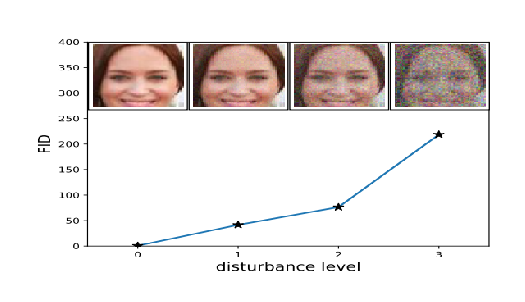
\includegraphics[scale=1.6]{figs/fid.eps}
     \caption{Plot of how FID scoring changes when Gaussian noise is added to the image \cite{fid}.}\label{Fig:FID}
 \end{figure}
 
Idea for the new metric is to use one of the last layers in the Inception model (pooling layer before classification output) to capture and encode specifics of an image. The output vector of this layer is of shape $(2048,)$ and is approximated by multivariate normal distribution. Set of these features is calculated for both real images and images generated by the model. We can denote the mean and covariance of embedded layer for generated images as, respectively, $\mu_{r}$ and  $\Sigma_{r}$. Same properties for real images are denoted as $\mu_{g}$ and $\Sigma_{g}$. Final score is calculated as a distance between the two data distributions, formally defined as

\begin{equation}
\operatorname{FID}(r, g)=\left\|\mu_{r}-\mu_{g}\right\|_{2}^{2}+\operatorname{tr}\left(\Sigma_{r}+\Sigma_{g}-2\left(\Sigma_{r} \Sigma_{g}\right)^{\frac{1}{2}}\right),
\end{equation}

\noindent Lower FID values indicate better generator performance, as the two distributions are \textit{closer} to each other. This score is more robust to noise than Inception Score - if generator only outputs small number of images per class (generated images are similar), the distance value between distributions will be high.


%%%%CLIP%%%%%%

\section{CLIP model}
%https://www.kdnuggets.com/2021/03/beginners-guide-clip-model.html
%https://openai.com/blog/clip/
\subsection{Overview}
\noindent In January 2021 OpenAI released new multi-modal model called \textbf{CLIP - Contrastive Language-Image Pre-Training}.  It is a neural network trained on $400 \;000 \;000$ image-text pairs - each pair is an image and its caption scrapped by OpenAI from the Internet. Main usage of the model is obtaining the most relevant text snippet for given image by using natural language embeddings and without directly optimizing for the task.
 \begin{figure}[ht!]
     \centering
     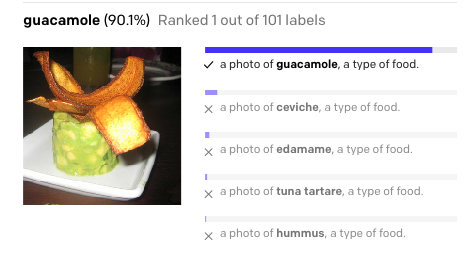
\includegraphics[scale=0.6]{figs/clip_example.png}
     \caption{Example of CLIP prediction. SOURCE}
 \end{figure}
\noindent CLIP is an example of \textbf{zero-shot} model.  That is, compared to commonly used classifiers that require custom datasets that represent target classes and don't generalize very well, CLIP can identify an enormous range of objects it has never seen before. OpenAI proves such functionality in the following table
\newline
 \begin{figure}[ht!]
     \centering
     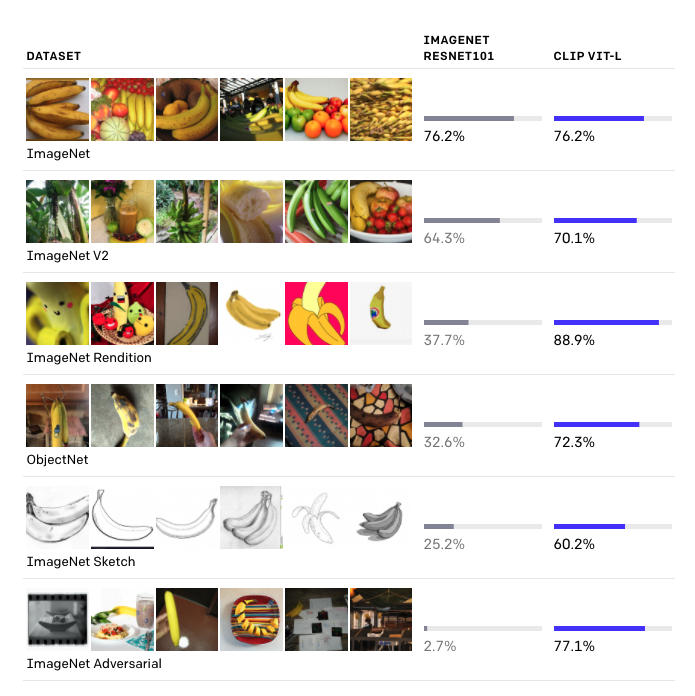
\includegraphics[scale=0.5]{figs/clip_summary.png}
     \caption{CAPTION AND SOURCE}
 \end{figure}
 \newpage
\noindent It compares ResNet101 model - trained on the ImageNet dataset with CLIP accuracy on different datasets.  It can be seen that for the ImageNet dataset, the accuracy is identical, but for the other models CLIP clearly provides better results and hence can be viewed as better generalizing model.
\newpage
\subsection{Methodology}
\noindent In order for images and text to be compared to one another, they must both be embedded.  Part of the CLIP model is responsible for embeddings -  it contains two encoders - ImageEncoder and TextEncoder.
 \begin{figure}[ht!]
     \centering
     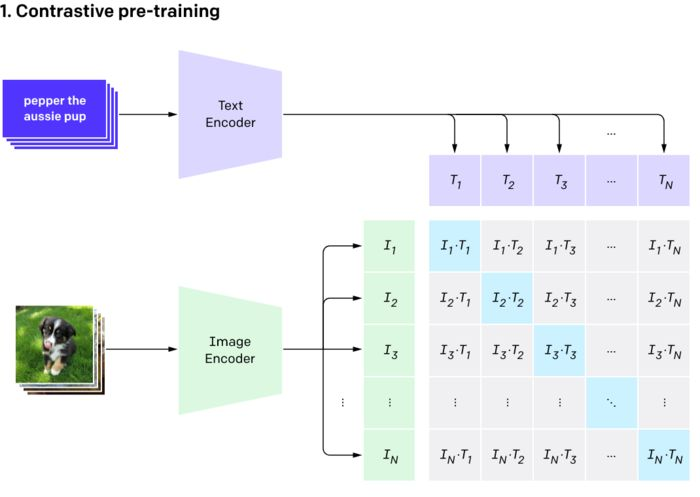
\includegraphics[scale=0.4]{figs/clip_model_1.jpeg}
     \caption{...}
 \end{figure}
 \newline
\noindent Image and text embeddings are compared in the similarity matrix $I \times T$ using \textbf{cosine similarity}:

\begin{equation}
\text{sim(\textbf{A}, \textbf{B})} = \frac{ \sum\limits_{i=1}^{n}{A_i  B_i} }{ \sqrt{\sum\limits_{i=1}^{n}{A_i^2}}  \sqrt{\sum\limits_{i=1}^{n}{B_i^2}} },
\end{equation}

\noindent where \textbf{A} and \textbf{B} are two vectors representing image and text embeddings respectively.

% \begin{definition}
%The cosine of two non-zero vectors can be derived by using the Euclidean vector dot product formula:
%
%$$\mathbf{A}\cdot\mathbf{B}
%=\left\|\mathbf{A}\right\|\left\|\mathbf{B}\right\|\cos\theta$$
%
%Given two vectors of attributes, $A$ and $B$, the cosine similarity, $\cos(\theta)$, is represented using a dot product and magnitude as
%
%$$\text{similarity} = \cos(\theta) = {\mathbf{A} \cdot \mathbf{B} \over \|\mathbf{A}\| \|\mathbf{B}\|} = \frac{ \sum\limits_{i=1}^{n}{A_i  B_i} }{ \sqrt{\sum\limits_{i=1}^{n}{A_i^2}}  \sqrt{\sum\limits_{i=1}^{n}{B_i^2}} }$$
%
%where $A_i$and $B_i$ are components of vector $A$ and $B$ respectively.
% \end{definition}

%\noindent During training, it is known, that the values on the diagonal represent correct classifications, so their similarity mus be higher than those in the same row/column. This approach contrast what we know go together (diagonal values) to what we know doesn’t go together (non-diagonal values). You can see that each row is a classification task: given an input image I, predict the text. Similarly, each column is a classification task: given an input text T, predict the image. During training, OpenAI used a very large size of mini-batches 32768 (N on the figure above). During inference one takes a set of labels, creates texts based on labels and runs these texts through the text encoder. Text embeddings are later matched to image representation.  \\

Model objective is to maximize cosine similarities for successive training (image, text) pairs and minimizing it for "negative" pairs - which means not training pairs. \\
One detail that is worth mentioning is that CLIP is sensitive to words used for image descriptions. Texts “a photo of a bird”, “a photo of a bird siting near bird feeder”, or “an image of a bird” all produce different probability paired with the same image:

 \begin{figure}[ht!]
     \centering
     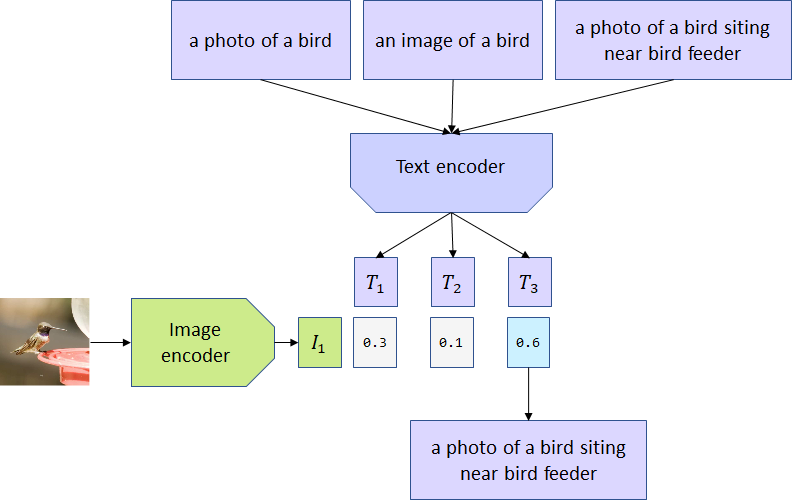
\includegraphics[scale=0.5]{figs/clip_model_3.png}
     \caption{CLIP is producing different probabilities for different bird image descriptions. SOURCE}
 \end{figure}
 \newpage
 \subsection*{Current results and limitations}
 
\noindent CLIP authors are open about its limitations. CLIP struggles on more abstract or systematic tasks such as counting the number of objects and on a more complex tasks such as estimating relative distances between objects. On such datasets, CLIP is only slightly better than random guessing. CLIP also struggles with very fine-grained classification, such as telling the difference between car models, variants of aircraft, or flower species.\\
\noindent What's more,  CLIP model itself is data hungry and expensive to train. If pre-trained model doesn’t work well for you, it may be not feasible to train your own version.\\
\noindent While zero-shot CLIP tries to reformulate classification task, the principles are still the same. And although CLIP generalizes well to many image distributions, it still generalizes poorly to data that is truly out-of-distribution. One example of this was CLIP’s performance on MNIST dataset where CLIP zero-shot accuracy was $88 \%.$ Logistic regression on raw pixels outperforms CLIP.\\
\noindent Ability to adapt to new datasets and classes is related to text encoder. It is thus limited to choosing from only those concepts known to the encoder. CLIP model trained with English texts will be of little help if used with texts in other languages. \\
\noindent Finally, CLIP’s classifiers can be sensitive to wording in label descriptions and may require trial and error to perform well.
\newpage
\section{Evolutionary Algorithms}

Evolutionary algorithms are a population-based heuristic methods of optimization. Algorithms from this family use computational implementations of processes related to natural selection, such as crossover, mutation and reproduction. Main idea of the algorithm is the \textit{survival of the fittest} principle inspired by Darwinian evolution theory, where main objective is to generate more and more \textit{fit} members of the population, while reducing the number of \textit{weak} units. That \textit{fitness} level is measured and described by \textit{fitness function}, which determines the quality of each population sample.

In the following sections we will describe main algorithms of our interest that we will apply for latent search problem. 
\subsection{Genetic Algorithm}

% pics from: https://www.sciencedirect.com/science/article/pii/S1364815218305905

The Genetic Algorithm is one of the first methods used and defined as evolutionary algorithm. It is still used with success until today and the number of variations and different applications of the method still grows.

 \begin{figure}[ht!]
     \centering
     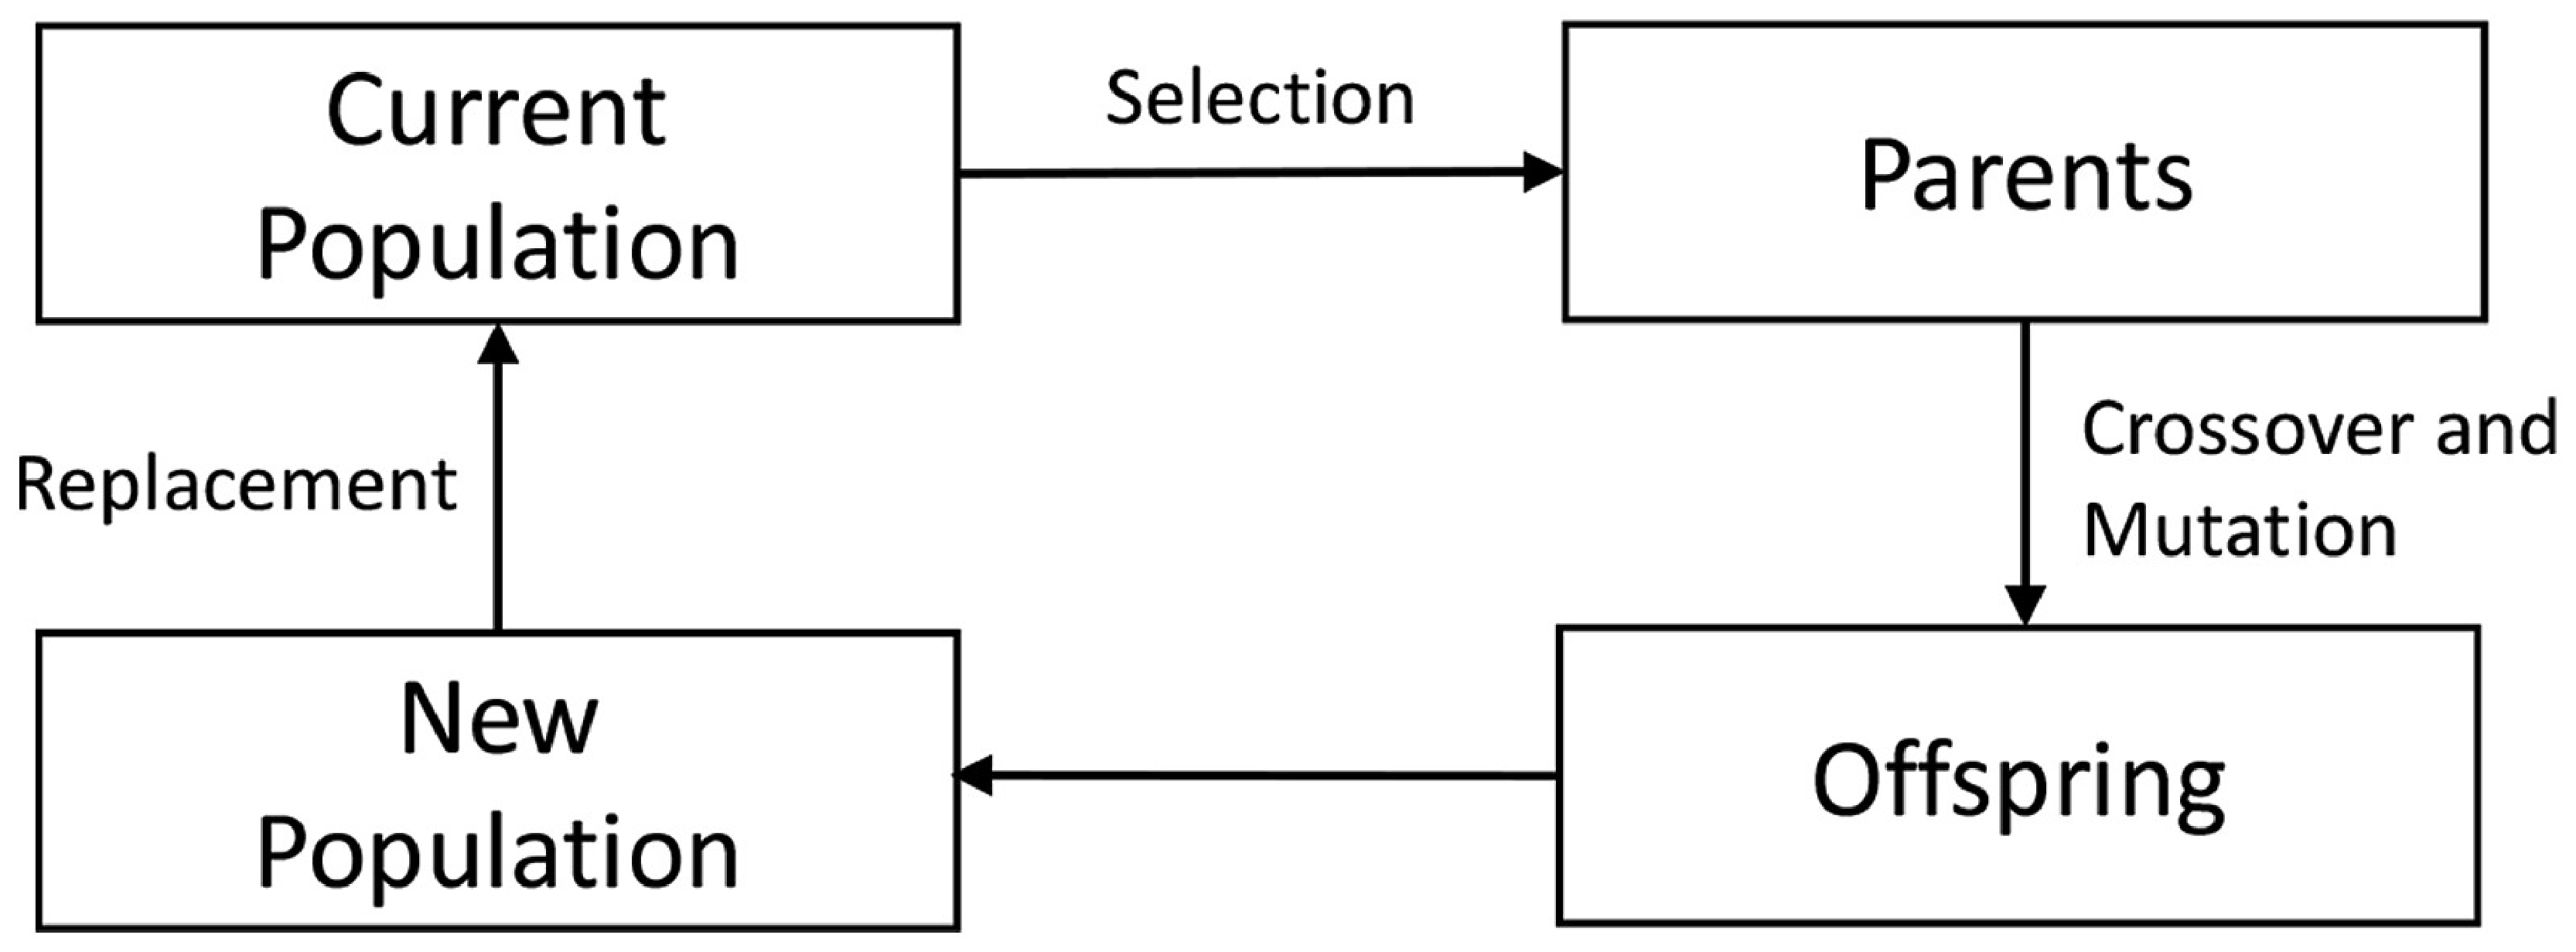
\includegraphics[scale=0.22]{figs/gen-algo.eps}
     \caption{Genetic algorithm optimization loop.}\label{Fig:genalgo1}
 \end{figure}


\noindent Standard genetic algorithm uses several operators for optimization purposes:

% Crossover is a process in which members of the last population are mated at random in the mating pool. So, a pair of offsprings is generated, combining elements from two parents (members), which hopefully have improved fitness values. Mutation is the occasional (with small probability) random alteration of the value of a string position. In fact, mutation is a process of random walk through the coded parameter space. Its purpose is to ensure that important information contained within strings may not be lost prematurely.

% Crossover operators may work for both intensification and diversification during the search, depending on the type of crossover operator and the locations of parents with respect to each other.

% Mutation operators is generally regarded as a random disturbance term of the individual chromosome, such that it can escape from the local area. 

% Uniform mutation that replaces the value of a decision variable by a uniformly distributed random number between the variable lower and upper bounds (R2 = random number in [x2l, x2u]). Example outcome of (c) single-point crossover and (d) uniform mutation in a 2D decision variable space.

% Mutation works to preserve and introduce diversity during the search. It enables the EA to escape local optima.

\begin{enumerate}
\item \textbf{Crossover} - process in which units from latest population are \textit{mixed} together at random. In this way, offsprings that come from the parents have combined features from both parents. It works for intensification and diversification of search, although it depends on the type of crossover operator and the location of the parents in the search space.
\item \textbf{Mutation} - these operators are widely regarded as introducing some random disturbance for individual units in the population. Uniform mutation replaces the value of a single decision variable by a value that is randomly selected from a space within lower and upper bound for given variable. This mainly introduces diversification and also helps to escape local optima.
\item \textbf{Replacement} - after performing crossover and mutation for given population, newly generated offspring are evaluated by the fitness function. Several (this number is usually dependent on the algorithm hyperparameters) newly created members with best score are placed in the population, the same number of worst units is removed.
\item \textbf{Selection} - the most promising units from population (members with best results regarding the fitness function) are chosen for mating. This generally promises the best chance to generate better units in the next population.
\end{enumerate}


 \begin{figure}[ht!]
     \centering
     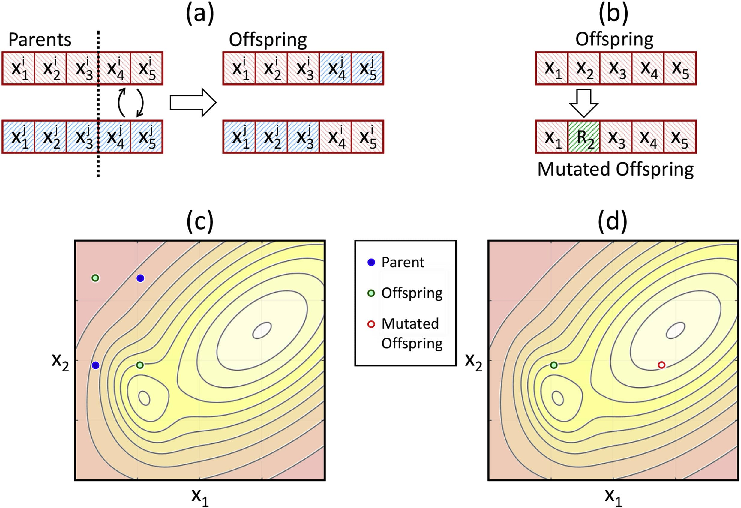
\includegraphics[scale=0.17]{figs/gen-algo-2.eps}
     \caption{Example of crossover and mutation operations.}\label{Fig:PROGAN}
 \end{figure}
 
The algorithm terminates based on several common criteria, most often when a solution is found that satisfies minimum criteria or when fixed number of generations is reached. Below is the pseudocode for the base genetic algorithm. 

 \begin{figure}[ht!]
     \centering
     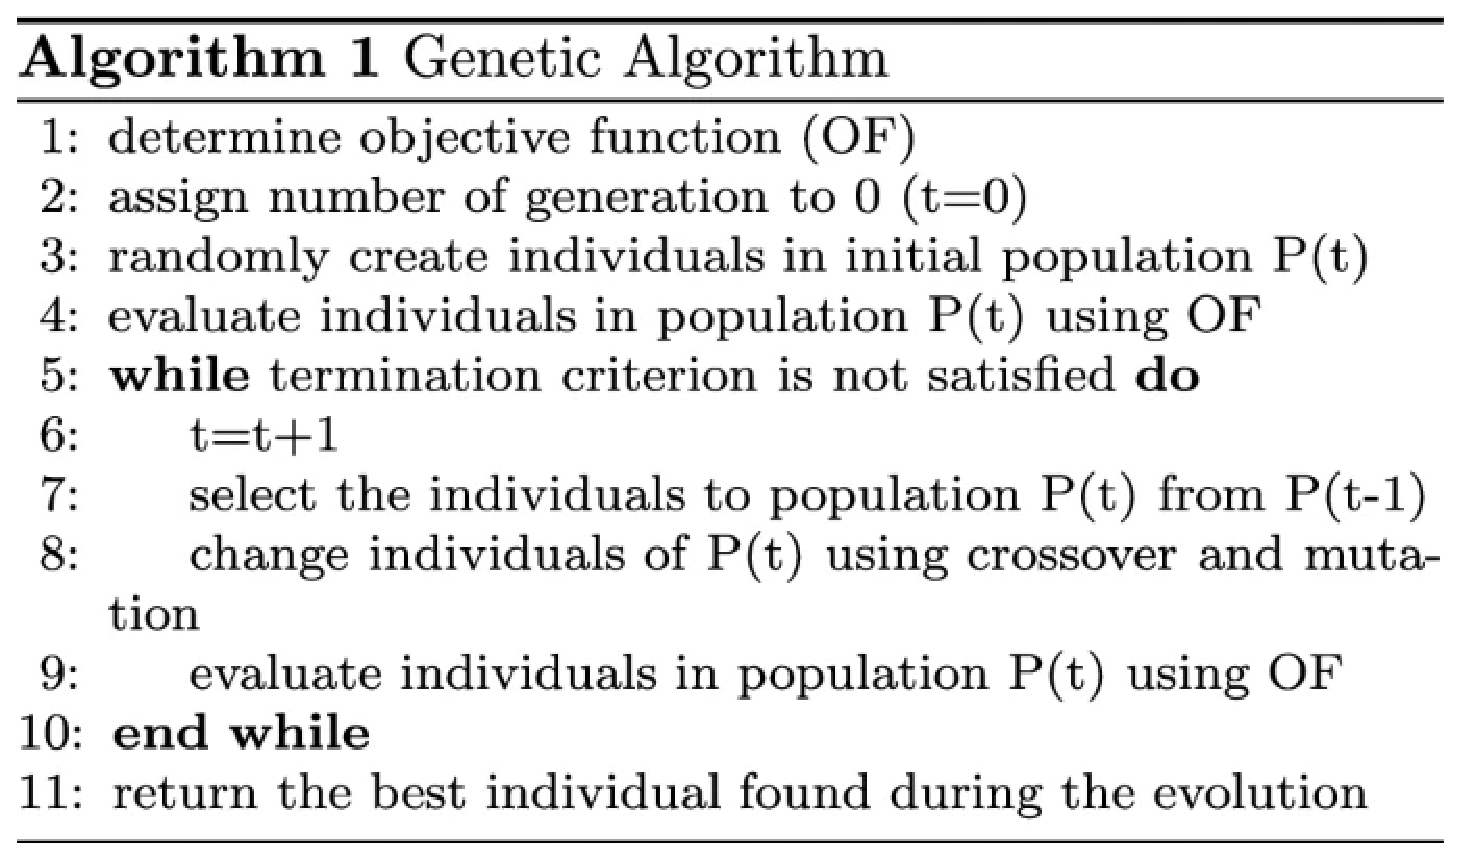
\includegraphics[scale=0.4]{figs/gen-algo-pseudo.eps}
     \caption{Genetic algorithm pseudocode.}\label{Fig:PROGAN}
 \end{figure}

% 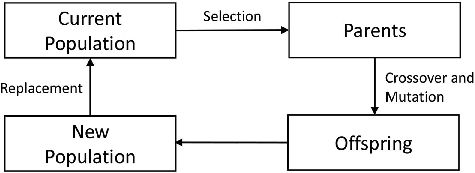
\includepdf[scale=0.5]{figs/gen-algo.pdf}

% The genetic algorithm (GA) [1] is one of the oldest and most known optimization techniques, which are based on nature. In the GA, the search for solution space imitates the natural process which takes place in the environment, and the Darwinian theory of species evolution is taken into consideration. In GAs, we have a population of individuals; each, called a chromosome, represents a potential solution to the problem. The problem being solved is defined by the objective function. Depending on how “good” the given individual is fitted to the objective function, the value which represents its quality is attributed to it. This value is referred to as the fitness of the individual, and it is a main evaluating factor. Highly valued individuals have a better chance to be selected to the new generation of the population. In GAs, we have three operators: selection (a new population of individuals is created based on the fitness values of individuals from the previous generation), crossover (typically parts of individuals are exchanged between two individuals selected to the crossover), and mutation (the values of particular genes are changed randomly). Algorithm 1 presents the standard GA in the pseudo-code form (for more details see [7]).

\subsection{Differential Evolution}

Differential evolution algorithm is a very efficient method most commonly used for optimization of function in continuous search space. It was proposed by Storn and Price in \cite{de}.

The main advantages over general genetic algorithm is more efficient memory usage, lower complexity and faster convergence.

 \begin{figure}[ht!]
     \centering
     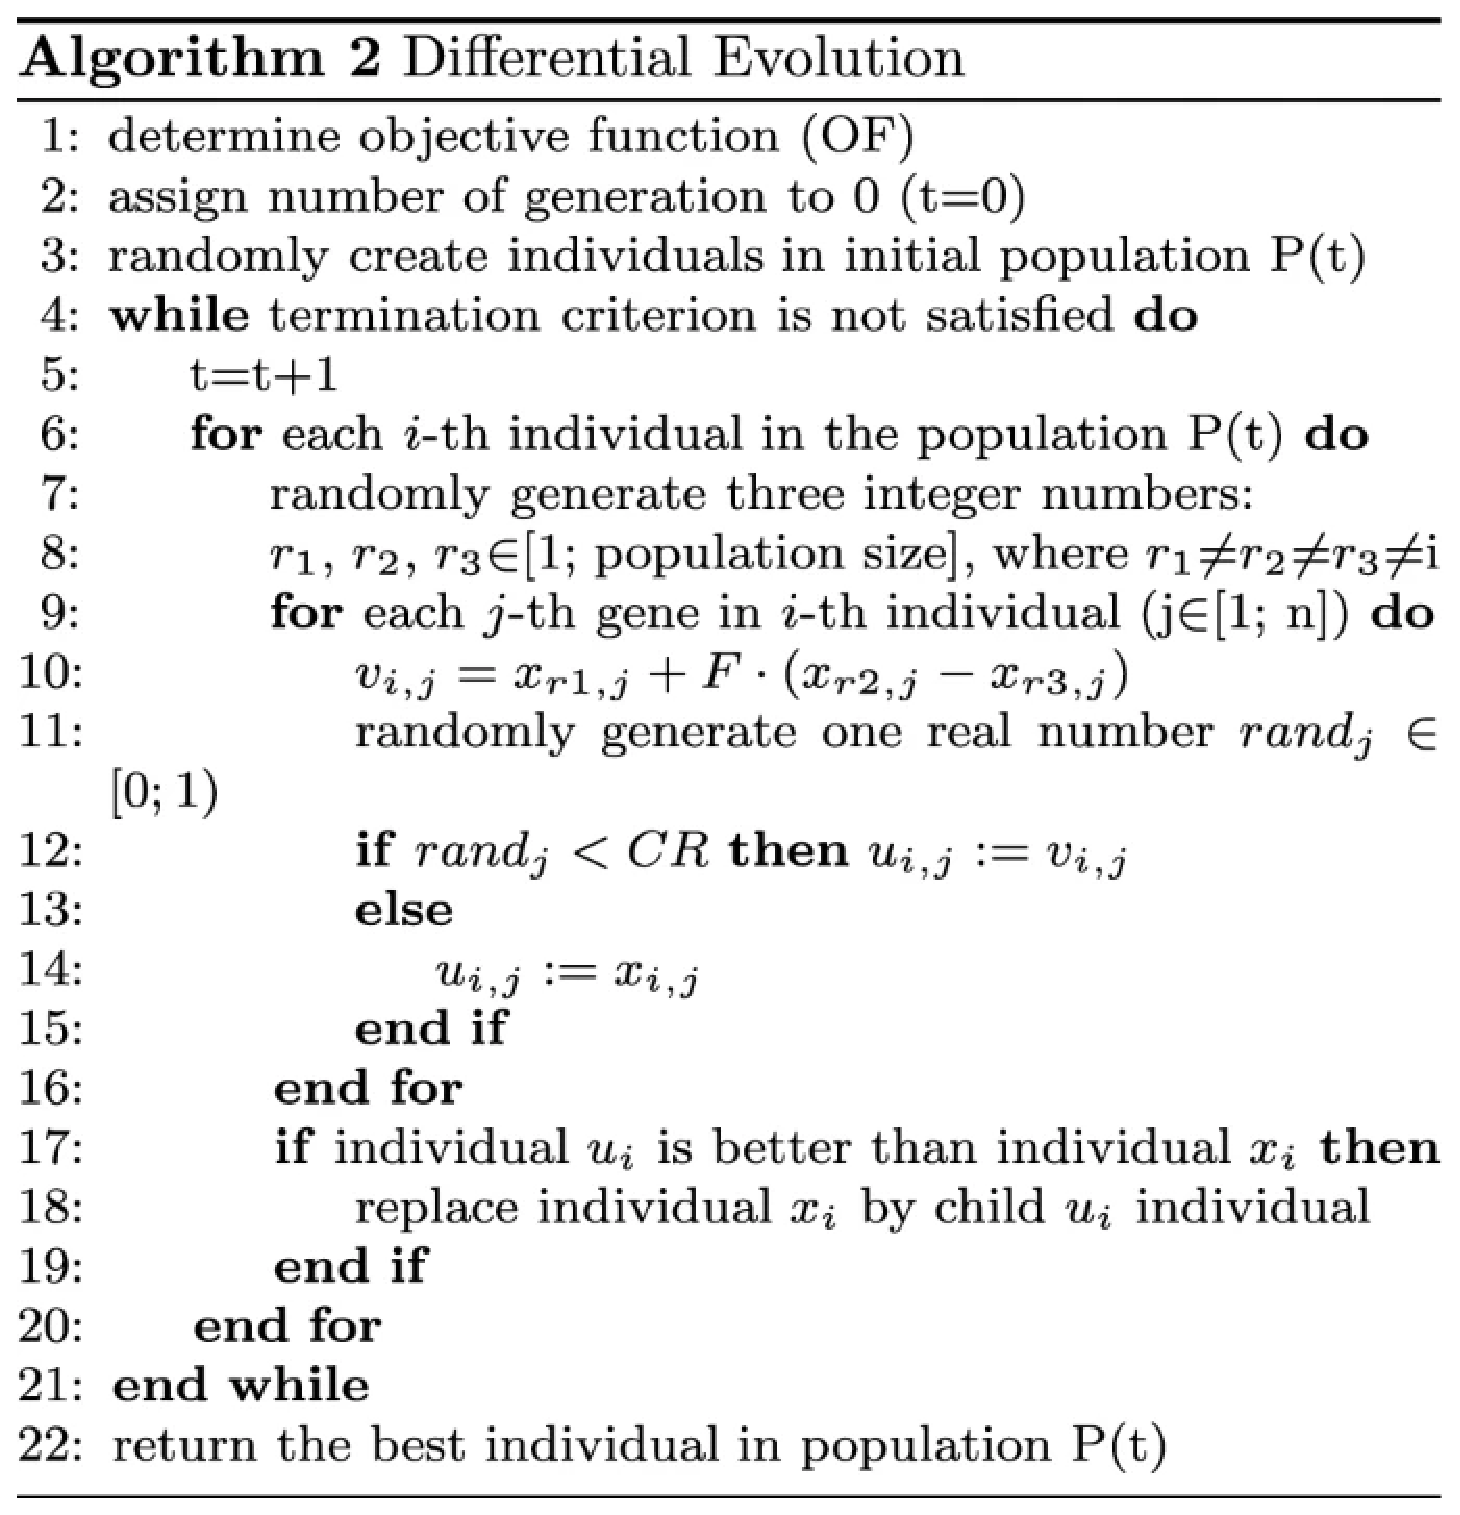
\includegraphics[scale=0.5]{figs/diff-evo.eps}
     \caption{Differential evolution DE/rand/1 pseudocode.}\label{Fig:PROGAN}
 \end{figure}

Below we will present the mathematical formulation of the algorithm and discuss most popular versions.

Differential evolution is primarily described by three parameters: $N_{p}$ - population size, $C_{r}$ - crossover control parameter and $F$ - scaling factor, also known as amplification parameter.\
Each member of every population is described as $D$-dimensional parameter vector. Each population in the algorithm can be understood as vector $\textbf{x}_{i, g}$, where $i \in \{1, 2, ..., N_{p}\}$ and $g$ stands for generation number.

\noindent Method incorporates usage of three vectors, which we will name for simplicity:

\begin{itemize}
\item Donor vector, which is created in the mutation step,
\item Trial vector, which is created in the crossover step,
\item Target vector, which is the vector of current population.
\end{itemize}


In the \textbf{mutation} step donor vector $v_{i, g}$ is produced. It is calculated by adding the scaled difference of two vectors to the third vector from the population. There are two most popular variations of mutation used in differential algorithm, one is the \textit{DE/rand/1} version, where all three vectors used in mutation are taken at random, which allows us to write a formula for donor vector  $v_{i, g}$ as

\begin{equation}
\mathbf{v}_{i, g}=\mathbf{x}_{r_{1}, g}+F\left(\mathbf{x}_{r_{2}, g}-x_{\mathbf{r}_{3}, g}\right),
\end{equation}

\noindent where $r_{1}, r_{2},r_{3} \in \{1, 2, ..., N_{p}\}$ are randomly selected indices and $F$ is the aforementioned scaling factor.

%The other choice is the \textit{DE/best/1} version, which chooses two random vectors to calculate the scaled value which is used to change the \textbf{best} vector $\mathbf{x}_{best, g}$ in current population, which results in more greedy version of the method
%
%\begin{equation}
%\mathbf{v}_{i, g}=\mathbf{x}_{best, g}+F\left(\mathbf{x}_{r_{2}, g}-x_{\mathbf{r}_{3}, g}\right).
%\end{equation}
%
%After the mutation algorithm performs \textbf{crossover} step. There are two most popular crossover schemes: binomial and exponential. Crossover step is performed using rate parameter $C_{r} \in \left(0, 1\right)$, which determines size of perturbation of the target vector. This influences the population diversity.\\
%\indent In binomial crossover, the trial vector $\mathbf{u}_{i, g}=\left(u_{i, 1, g}, u_{i, 2, g}, \ldots, u_{i, D, g}\right)$ for $i \in \{1, 2, ..., N_{p}\}$ and $j \in \{1, 2, ..., D\}$ is created using formula
%
%\begin{equation}
%u_{i, j, g}=\left\{\begin{array}{ll}
%v_{i, j, g} & \text{if } rand_{j} \leqslant C_{r} \text { or } j=j_{\mathrm{rd}}, \\
%x_{i, j, g} & \text { otherwise,}
%\end{array}\right.
%\end{equation}
%
%\noindent where $rand_{j}$ is a random number from $(0,1)$ which determines the probability that the $j$-th parameter will crossover and $\mathbf{v}_{i, g}$ is the donor vector calculated in the mutation step. Also, $j_{\mathrm{rd}}$ is a randomly chosen integer in the range $[1, D]$, which ensures that at least one parameter will be chosen for crossover. That ensures that the new population will be always different from previous one.\
%
%For exponential crossover scheme, let us define the indices $a$ and $b$ to be chosen independently and at random from $[1, D]$. These parameters are chosen for each trial vector separately. Let's denote $\left(\right)_{MOD_{D}}$ as modulo function with modulus $D$. Using these we can define a set of indices
%\begin{equation}
%I = \left\lbrace a, \left(a+1\right)_{MOD_{D}}, \ldots, \left(a+b-1\right)_{MOD_{D}}\right\rbrace.
%\end{equation}
%The trial vector $\mathbf{u}_{i, g}=\left(u_{i, 1, g}, u_{i, 2, g}, \ldots, u_{i, D, g}\right)$ for $i \in \{1, 2, ..., N_{p}\}$ and $j \in \{1, 2, ..., D\}$ is created as
%\begin{equation}
%u_{i, j, g}=\left\{\begin{array}{cc}
%v_{i, j, g} & \text {if } j \in I \text { and } rand_{j} \leqslant C_{r}, \\
%x_{i, j, g} & \text { otherwise. }
%\end{array}\right.
%\end{equation}
%
%\noindent Essentially, above formula is focusing on the crossover between neighbouring vector features instead of fully randomizing the choice.\\
%Having produced a trial vector we can proceed to the selection step. In this phase, algorithm is greedily choosing new members of the population using the \textit{fitness function} $f$.
%
%\begin{equation}
%\mathbf{x}_{i+1, g}=\left\{\begin{array}{ll}
%\mathbf{u}_{i, g} & \text {if } f\left(\mathbf{u}_{i, g}\right)<f\left(\mathbf{x}_{i, g}\right), \\
%\mathbf{x}_{i, g} & \text { otherwise }
%\end{array}\right.
%\end{equation}
%
%The algorithm terminates on similar basis as genetic algorithm discussed previously, when a optimal solution below certain treshold is found or when algorithm reaches some defined number of generations.


%
%Crossover: DE crossover strategies control the
%number of inherited components from the mutant
%vector to form a target vector. Binomial and exponential are main crossover schemes 16, 31. The
%DE crossover rate parameter Cr
%influences the size
%of the perturbation of the base (target) vector to
%ensure the population diversity 17
%.
%Binomial crossover: In the crossover operation
%of DE algorithm, a trial vector is formed. In the
%binomial crossover scheme, the trail vector ui,g =
%〈ui,1,g
%, ui,2,g
%, . . . , ui,D,g
%〉 is generated by the equation,
%for i = 1, 2, . . . ,Np
%, j = 1, 2, . . . , D


%
%DE algorithm has three different parameters: a
%population of size Np
%, a crossover control parameter
%Cr
%, and a difference vector amplification parameter
%F. Each population member in DE is represented
%as a D-dimensional parameter vector. In DE algorithm, the population is initialized randomly and is
%supposed to cover the entire search space. Each
%vector in the DE is represented by xi,g
%, where i =
%1, 2, 3, . . . ,Np and g is generation number. New
%offsprings in DE algorithm are generated by mutation, crossover, and selection operators. The repair
%operator proposed by Wang 30 is also used in th
%




%
%source:
%Storn, R., and Price, K. (1995). Differential Evolution—A Simple and Efficient Adaptive Scheme for Global Optimization Over Continuous Spaces. Technical Report, Berkeley, CA. Available online at: https://www.icsi.berkeley.edu/ftp/global/global/pub/techreports/1995/tr-95-012.pdf

% Differential evolution [3, 4], or DE, is a relatively recent EA formulation which uses a mechanism for
% adaptive search that does not make use of probability distributions. Whilst its basic mechanism is
% similar to a GA, its mutation operator is quite different, using a geometric approach that is motivated
% by the moves performed in the Nelder Mead simplex search method. This involves selecting two
% existing search points from the population, taking their vector difference, scaling this by a constant F,
% and then adding this to a third search point, again sampled randomly from the population. Following
% mutation, DE’s crossover operator recombines the mutated search point (the mutant vector) with
% another existing search point (the target vector), replacing it if the child solution (known as a trial
% vector) is of equal or greater objective value. There are two standard forms of crossover [5]:
% exponential crossover and binomial crossover, which closely resemble GA two-point crossover and
% uniform crossover, respectively. The comparisons between target vector and trial vector play the same
% role as the selection mechanism in a GA or ES. Since DE requires each existing solution to be used
% once as a target vector, the whole population is replaced in the course of applying crossover.
% An advantage of using simplex-like mutations in DE is that the algorithm is largely self-adapting,
% with moves automatically becoming smaller in each dimension as the population converges. More
% generally, the authors of the method have claimed that this sort of self-adaptation means that the size
% and direction of moves are automatically matched to the search landscape, a phenomenon they term
% contour matching. When compared to CMA-ES, for example, this means that the algorithm has few
% parameters and is relatively easy to implement.

%%%The differential evolution (DE) is a type of evolutionary algorithm useful mainly for the function optimization in continuous search space. Although a version of DE algorithm for combinatorial problems has also been discussed [51], the principal version of the DE algorithm was discussed by Storn and Price [3]. The main advantages of DE over a traditional GA are: It is easy to use, and it has efficient memory utilization, lower computational complexity (it scales better when handling large problems), and a lower computational effort (faster convergence) [52]. The standard DE procedure is shown in Algorithm 2. Presented there DE optimizes the problem with n decision variables. Parameter F scales the values added to the particular decision variables (mutation), and CR parameter represents the crossover rate [52] (xi,j is the value of jth decision variable stored in ith individual in the population). More detailed information on how the parameters should be tuned can be found in [53]. The main idea of the DE algorithm is connected with computing the difference between two individuals chosen randomly from the population. (The DE determines the function gradient within a given area—not at a single point.) Therefore, the DE algorithm prevents the solution of sticking at a local extreme of the optimized function [52]. Twenty years of DE development resulted in many modifications. Some of them are shortly presented in Table 1.


% n computational intelligence (CI), an evolutionary algorithm (EA) is a subset of evolutionary computation,[1] a generic population-based metaheuristic optimization algorithm. An EA uses mechanisms inspired by biological evolution, such as reproduction, mutation, recombination, and selection. Candidate solutions to the optimization problem play the role of individuals in a population, and the fitness function determines the quality of the solutions (see also loss function). Evolution of the population then takes place after the repeated application of the above operators.

% Evolutionary algorithms are a heuristic-based approach to solving problems that cannot be easily solved in polynomial time, such as classically NP-Hard problems, and anything else that would take far too long to exhaustively process. When used on their own, they are typically applied to combinatorial problems; however, genetic algorithms are often used in tandem with other methods, acting as a quick way to find a somewhat optimal starting place for another algorithm to work off of.
% The premise of an evolutionary algorithm (to be further known as an EA) is quite simple given that you are familiar with the process of natural selection. An EA contains four overall steps: initialization, selection, genetic operators, and termination. These steps each correspond, roughly, to a particular facet of natural selection, and provide easy ways to modularize implementations of this algorithm category. Simply put, in an EA, fitter members will survive and proliferate, while unfit members will die off and not contribute to the gene pool of further generations, much like in natural selection.

% Evolutionary algorithms (EAs) are population-based metaheuristics. Historically, the design of EAs
% was motivated by observations about natural evolution in biological populations. Recent varieties of
% EA tend to include a broad mixture of influences in their design, although biological terminology is
% still in common use. The term ‘EA’ is also sometimes extended to algorithms that are motivated by
% population-based aspects of EAs, but which are not directly descended from traditional EAs, such as
% scatter search. The term evolutionary computation is also used to refer to EAs, but usually as a
% generic term that includes optimisation algorithms motivated by other natural processes, such as
% particle swarm optimisation and artificial immune systems. Although these algorithms often resemble
% EAs, this is not always the case, and they will not generally be discussed in this chapter. For a
% discussion of their commonalities and differences, the reader is referred to [1].
% Over the years, EAs have become an extremely rich and diverse field of study, and the sheer number
% of publications in this area can create challenges to people new to the field. To address this, this
% chapter aims to give a concise overview of EAs and their application, with an emphasis on
% contemporary rather than historical usage.


\chapter{Notable architectures}
\section{StyleGAN}

StyleGAN is an architecture proposed by NVIDIA team in \cite{stylegan}. It is considered to be one of the most important publications regarding image generation and it introduces several novelties comparing to models used so far. It used several mechanisms (such as adaptive instance normalization and merging regularization) to generate highly realistic images with great resolution. It is greatly inspired by direct predecessor - Progressive Growing GAN architecture (called ProGAN), also published by NVIDIA.

\begin{figure}[ht!]
    \centering
    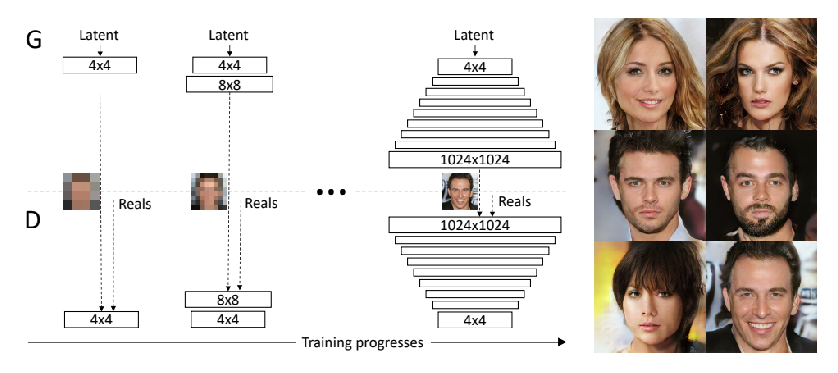
\includegraphics[scale=1.0]{figs/progan-scheme.eps}
    \caption{Progressive growing technique used in ProGAN.}\label{Fig:PROGAN}
\end{figure}

Most important idea presented in the ProGAN architecture, utilized also in StyleGAN, is the progressive structure of learning. Volume of generated by network images is growing from small resolution (starting at 4x4 pixels) to high resolution (up to 1024x1024 pixels) by upsampling. This training principle helps the network to solve simpler task before attending to generate a full-resolution image. It has been proven to help with stability of the training and reduce drastic abnormalities in final image.

\subsection{Architecture overview}

\begin{figure}[ht!]
    \centering
    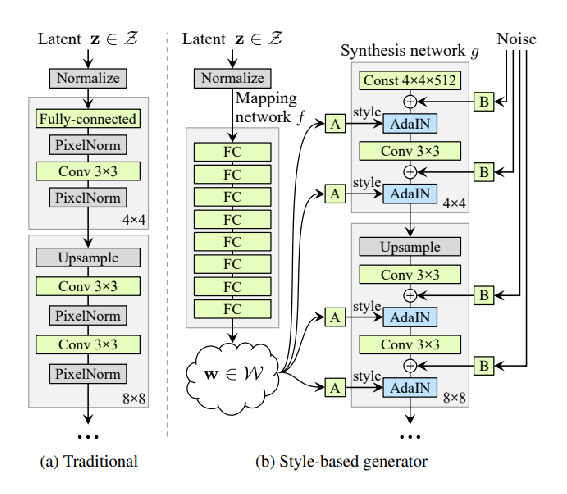
\includegraphics[scale=1.5]{figs/stylegan-scheme.eps}
    \caption{ProGAN and StyleGAN networks comparison.}\label{Fig:STYLEGAN}
\end{figure}


\subsection{Mapping network}

In the StyleGAN architecture authors introduced a intermediate layer between an input (latent vector $z \in \mathbb{Z}$) and the network called mapping layer (fig...). It works by applying 8 fully connected layers to the input and therefore encoding it as a new vector $w \in \mathbb{W}$. Main purpose of this procedure is to have better control over generative power of the model by separating elements of the vector that will be responsible for different image features.


\begin{figure}[ht!]
    \centering
    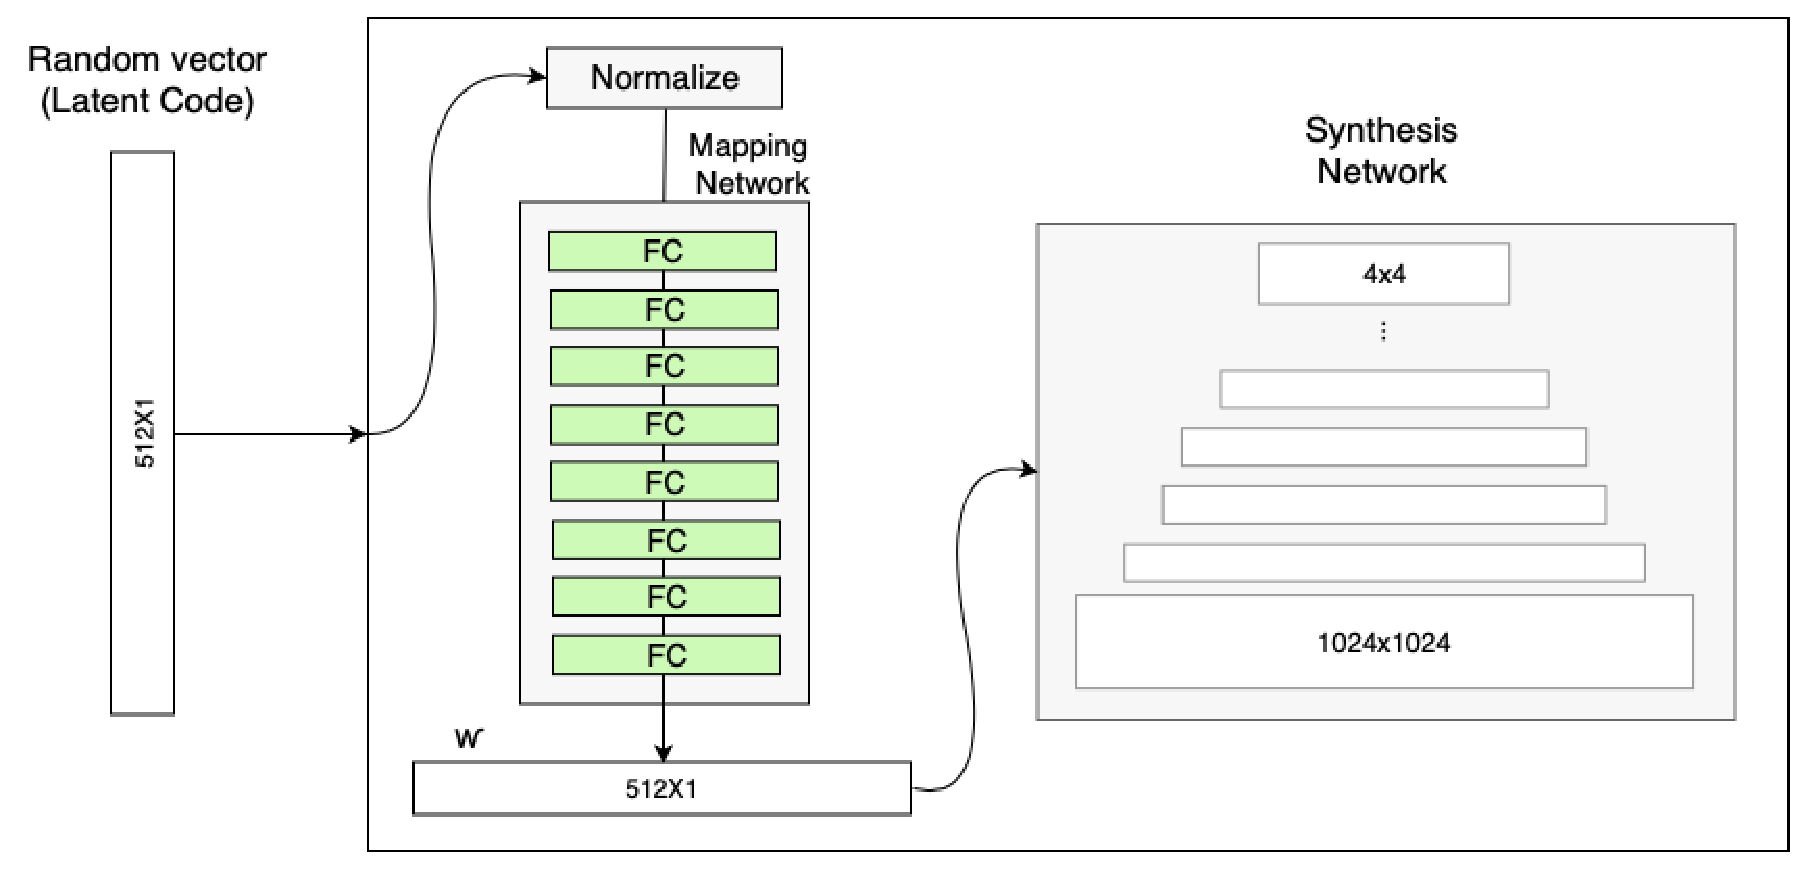
\includegraphics[scale=0.3]{figs/mapping-network.eps}
    \caption{Mapping network of StyleGAN.}\label{Fig:STYLEGAN}
\end{figure}


A common problem for generative models is a phenomenon called \textbf{feature entanglement}. We can consider a scenario where training is done on a dataset of human faces. It is very likely that most of the women in the dataset will have long hair and most men - short hair. This would result in the entanglement of \textit{hair length} and \textit{gender} features. Therefore, when latent vector is manipulated in order to change the hair length - the model will also change the gender of a person on the image, as it is associating these two occurencies as bounded together. The mapping layer is separating these features, allowing to change different elements of new vector $w$ without losing the integrity of an image.

\subsection{Adaptive Instance Normalization}

% https://arxiv.org/pdf/1703.06868.pdf - paper
% https://arxiv.org/pdf/1607.08022.pdf%7B - fast style transfer paper
% https://www.coursera.org/lecture/build-better-generative-adversarial-networks-gans/adaptive-instance-normalization-adain-cr6bv - explained
% https://towardsdatascience.com/light-on-math-machine-learning-intuitive-guide-to-neural-style-transfer-ef88e46697ee - style transfer

In the traditional generator, latent code is introduced to the network only in the first layer. The authors of StyleGAN are using the vector $w$ produced via mapping network to steer the style of an image at each convolutional layer by using \textbf{Adaptive Instance Normalization (AdaIN)} technique.

\begin{equation}
\operatorname{AdaIN}\left(\mathbf{x}_{i}, \mathbf{y}\right)=\mathbf{y}_{s, i} \frac{\mathbf{x}_{i}-\mu\left(\mathbf{x}_{i}\right)}{\sigma\left(\mathbf{x}_{i}\right)}+\mathbf{y}_{b, i},
\end{equation}

%% HERE THE EQUATION FOR ADAIN
%\begin{figure}[ht!]
%    \centering
%    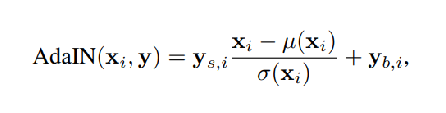
\includegraphics[scale=1.2]{figs/adain.eps}
%    \caption{Mapping network of StyleGAN.}\label{Fig:STYLEGAN}
%\end{figure}

The middle part of the equation is the \textbf{Instance Normalization (IN)}. Each channel of the convolution layer is normalized. Values $\textbf{y}_{s,i}$ and $\textbf{y}_{b,i}$ are calculated from the vector $v$ using fully-connected layer and correspond to \textit{A} on the figure-main one. These can be understood as scale and bias; these values are used to translate the information from vector $w$ to a feature map generated by convolution.

\begin{figure}[ht!]
    \centering
    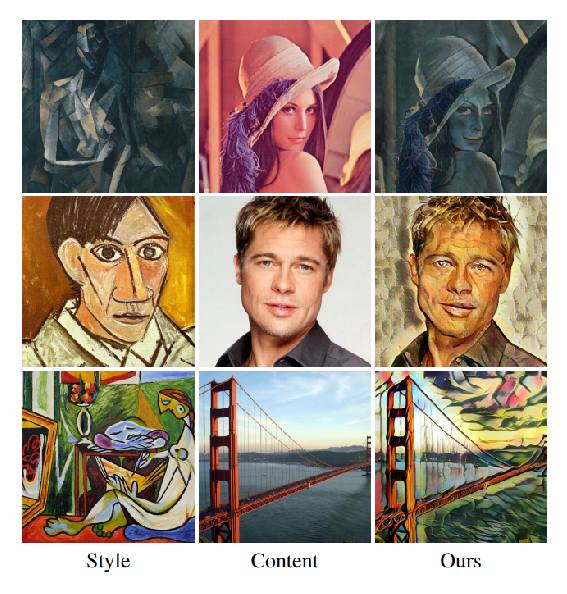
\includegraphics[scale=1.0]{figs/adaptive-instance-norm.eps}
    \caption{Example of AdaIN application for style transfer.}\label{Fig:STYLEGAN}
\end{figure}

Adding this method of including latent vector at every step of network computation resulted in drastic improvement of network's performance which can be see in the table below.

\begin{figure}[ht!]
    \centering
    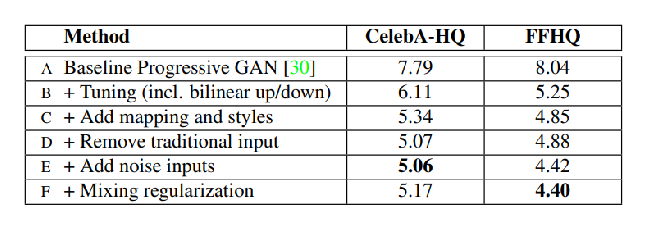
\includegraphics[scale=1.2]{figs/frechet-distance.eps}
    \caption{Mapping network of StyleGAN.}\label{Fig:STYLEGAN}
\end{figure}


%%%% NOTES %%%%

% This normalization is called \textit{adaptive}, because 

% Main task of this structure is elastic 

% where the input feature map is normalized with instance normalization first. Then, StyleGAN scales and biases each normalized spatial feature map by the style information. (μ and σ are the mean and the standard deviation of the input feature map xᵢ respectively.) In each layer, StyleGAN computes a pair of style values (y(s, i) and y(b, i)) as the scale and the bias from w to apply the style to the spatial feature map i. The normalized feature influences the amount of style applied to a spatial location.


% The AdaIN (Adaptive Instance Normalization) module transfers the encoded information ⱳ, created by the Mapping Network, into the generated image. The module is added to each resolution level of the Synthesis Network and defines the visual expression of the features in that level:
% Each channel of the convolution layer output is first normalized to make sure the scaling and shifting of step 3 have the expected effect.
% The intermediate vector ⱳ is transformed using another fully-connected layer (marked as A) into a scale and bias for each channel.
% The scale and bias vectors shift each channel of the convolution output, thereby defining the importance of each filter in the convolution. This tuning translates the information from ⱳ to a visual representation.


% While a traditional generator [30] feeds the latent code
% though the input layer only, we first map the input to an intermediate latent space W, which then controls the generator
% through adaptive instance normalization (AdaIN) at each convolution layer. Gaussian noise is added after each convolution, before evaluating the nonlinearity. Here “A” stands for a learned
% affine transform, and “B” applies learned per-channel scaling factors to the noise input. T



% Mapping Network
% The Mapping Network’s goal is to encode the input vector into an intermediate vector whose different elements control different visual features. This is a non-trivial process since the ability to control visual features with the input vector is limited, as it must follow the probability density of the training data. For example, if images of people with black hair are more common in the dataset, then more input values will be mapped to that feature. As a result, the model isn’t capable of mapping parts of the input (elements in the vector) to features, a phenomenon called features entanglement. However, by using another neural network the model can generate a vector that doesn’t have to follow the training data distribution and can reduce the correlation between features.
% The Mapping Network consists of 8 fully connected layers and its output ⱳ is of the same size as the input layer (512×1).

% Mapping Network moreover Style Network: The purpose of the mapping network is to produce the latent input vector within the intermediate vector whose distinctive element control various visual features. Instead of immediately implementing latent vector to the input layer, mapping is done.

% The main principle behind training the StyleGAN is this “progressive” method which was first used by NVIDIA in their ProGAN. It works by gradually increasing the resolution , thus ensuring that the network evolves slowly, initially learning a simple problem before progressing to learning more complex problems(or, in this case, images of a higher resolution). This kind of training principle ensure stability and has been proven to minimize common problems associated with GANs such as mode collapse. It also makes certain that high level features are worked upon first before moving on to the finer details, reducing the likelihood of such features being generated wrong(which would have a more drastic effect on the final image than the other way around). StyleGANs use a similar principle, but instead of generating a single image they generate multiple ones, and this technique allows for styles or features to be dissociated from each other.

% Baseline Progressive Growing GANs: Style GAN uses baseline progressive GAN structure, which means the volume of the generated picture increases progressively from a shallow resolution (4×4) to high resolution (1024 x1024) by adding a new section to both the models to maintain the larger resolution after applying the model on a more modest resolution to make it further stable.

As additional technique of regularization and method to differentiate the generated images further, a \textbf{style mixing} approach was introduced by the authors. The main idea is to use not one but two (or more) latent vectors $w_{1}, w_{2}$ (obtained from mapping of $z_{1}, z_{2}$) to generate the final image. The way in which mixing is introduced is fairly simple; up to certain point in the architecture vector $w_{1}$ is used for style control and from crossover point vector $w_{2}$ is used.
Depending on the place of crossover, final image obtains different characteristics from each image. 
%
%
%\subsection{Additional noise inputs}
%
%Authors provided the generator with ability to alternate very fine details on a picture by adding stochastic variance into the model. Single-channel images of uncorrelated Gaussian noise are fed into different places in the architecture. Noise is scaled per channel (which means that the amount of noise is a learnable parameter) and added after each convolution layer before AdaIN layer.
%
%\begin{figure}[ht!]
%    \centering
%    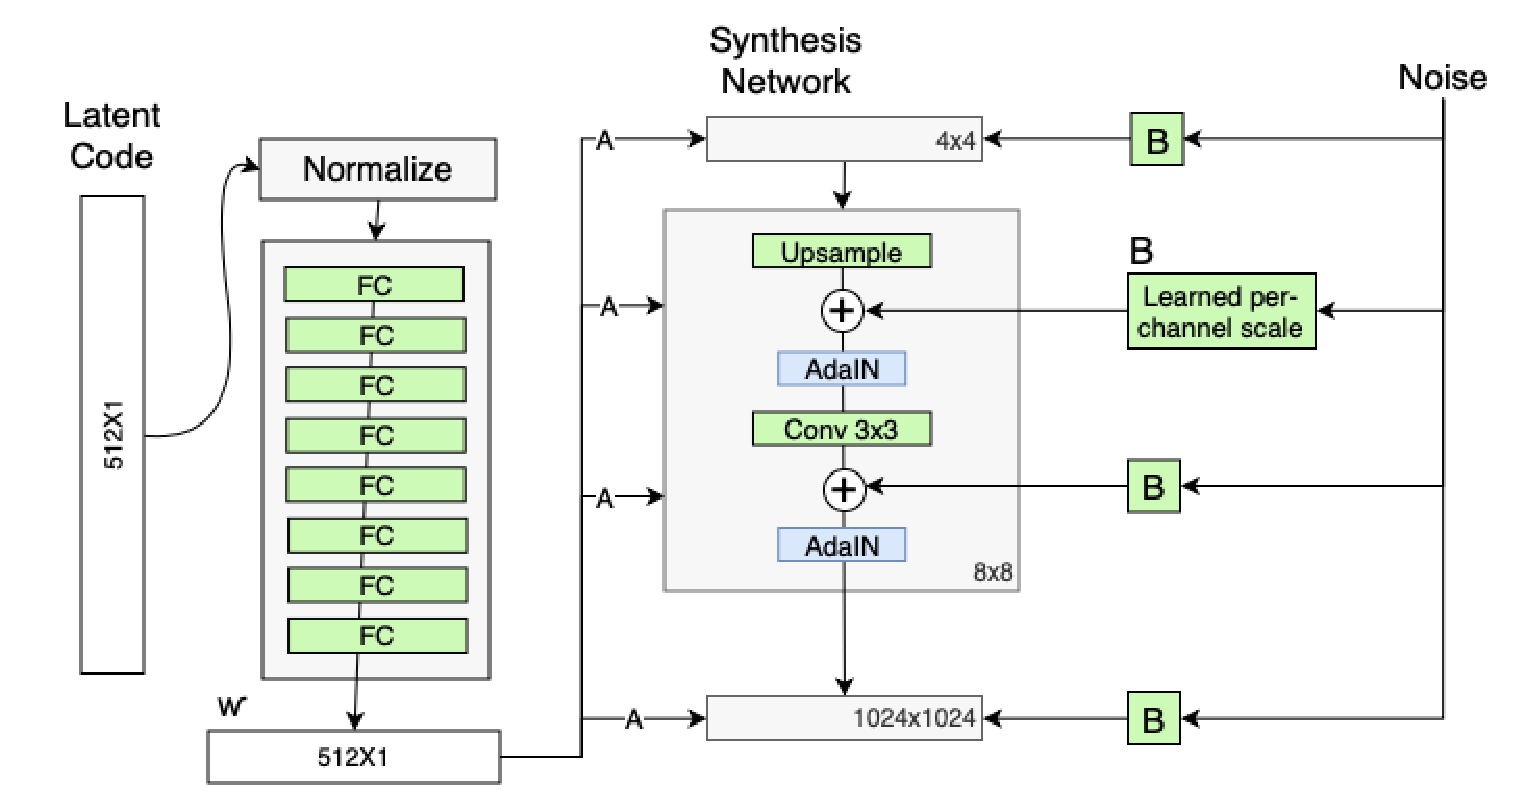
\includegraphics[scale=0.5]{figs/noise.eps}
%    \caption{Places in the architecture where noise is added.}\label{Fig:STYLEGAN}
%\end{figure}
%
%Additional noise allows to generate and alternate very detailed parts of the image (wrinkles, freckles, hair). Thanks to scalability and DOKONCZYC
%
%\begin{figure}[ht!]
%    \centering
%    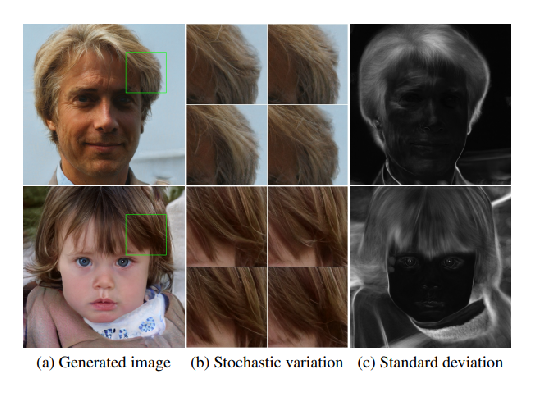
\includegraphics[scale=1.4]{figs/stochastic-variation.eps}
%    \caption{Visual inspection of where the gaussian noise tends to be the most active.}\label{Fig:STYLEGAN}
%\end{figure}

% Gaussian noise is added after each convolution, before evaluating the nonlinearity. Here “A” stands for a learned
% affine transform, and “B” applies learned per-channel scaling factors to the noise input.

% Finally, we provide our generator with a direct means
% to generate stochastic detail by introducing explicit noise
% inputs. These are single-channel images consisting of uncorrelated Gaussian noise, and we feed a dedicated noise
% image to each layer of the synthesis network. The noise
% image is broadcasted to all feature maps using learned perfeature scaling factors and then added to the output of the
% corresponding convolution, as illustrated in Figure 1b. The
% implications of adding the noise inputs are discussed in Sections 3.2 and 3.3.


% There are many aspects in people’s faces that are small and can be seen as stochastic, such as freckles, exact placement of hairs, wrinkles, features which make the image more realistic and increase the variety of outputs. The common method to insert these small features into GAN images is adding random noise to the input vector. However, in many cases it’s tricky to control the noise effect due to the features entanglement phenomenon that was described above, which leads to other features of the image being affected.
% The noise in StyleGAN is added in a similar way to the AdaIN mechanism — A scaled noise is added to each channel before the AdaIN module and changes a bit the visual expression of the features of the resolution level it operates on.


\section{StyleGAN2}

Significant improvements of the StyleGAN architecture were proposed in late 2019. Publication revolved mainly around the problems which emerged during StyleGAN generator. It has been noticed that several parts of the network cause imperfections in the final images, which are called \textit{artifacts}. Two main types of artifacts were formulated in the paper:

\begin{itemize}
\item \textbf{Water-droplet artifacts} - the blob-shaped characteristics that resemble water-droplets are visible in various places in the final images. It might not be obvious while looking at the image, but it is very visible in the intermediate feature maps produced by generator. This artifacts starts to appear around 64x64 pixels resolution and gets stronger with higher resolutions. 
\item \textbf{Phase artifacts} - output images show strong location preference for several features e.g. facial features like teeth or eyes. This causes some of the features to remain unchanged when major components of the image such as pose or rotation are vastly different.
\end{itemize}


\begin{figure}[ht!]
    \centering
    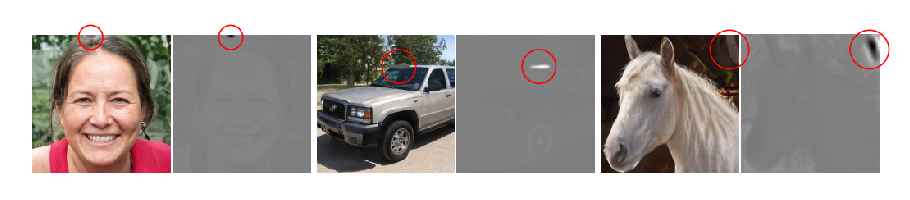
\includegraphics[scale=1.0]{figs/water-droplets.eps}
    \caption{Water droplets artifact and its effect on feature maps.}\label{Fig:STYLEGAN}
\end{figure}



\begin{figure}[ht!]
    \centering
    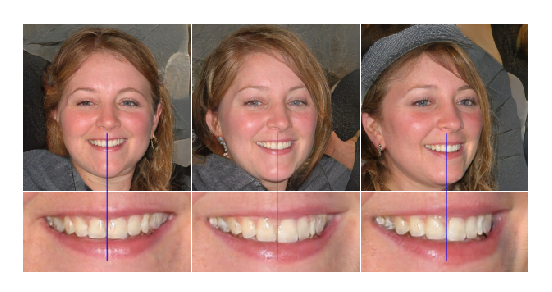
\includegraphics[scale=1.2]{figs/phase.eps}
    \caption{Phase artifact. Blue line helps to visualize that teeth are staying in the same place even with changing a significant feature of image such as rotation of the face..}\label{Fig:STYLEGAN}
\end{figure}

\subsection{Architecture overview}

\begin{figure}[ht!]
    \centering
    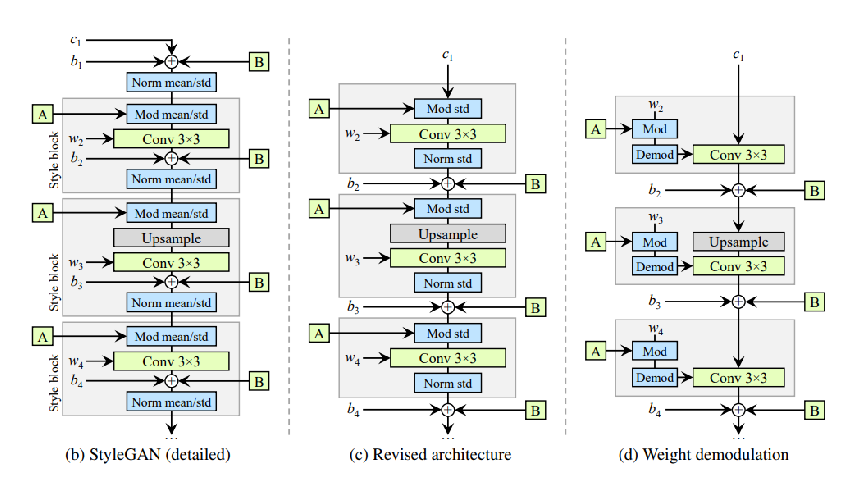
\includegraphics[scale=1.0]{figs/stylegan2-scheme2.eps}
    \caption{Visual inspection of where the gaussian noise tends to be the most active.}\label{Fig:STYLEGAN}
\end{figure}


\subsection{Revisiting Instance Normalization}

The water-droplet effect was speculated to be a side effect of AdaIN method applied in the style blocks. Authors pointed out that this type of normalization affects each feature map separately (works independently for every channel) and potentially destroys meaningful information that is included in the differences between feature maps values.

To address this problem, significant changes to the architecture were proposed.

\begin{figure}[ht!]
    \centering
    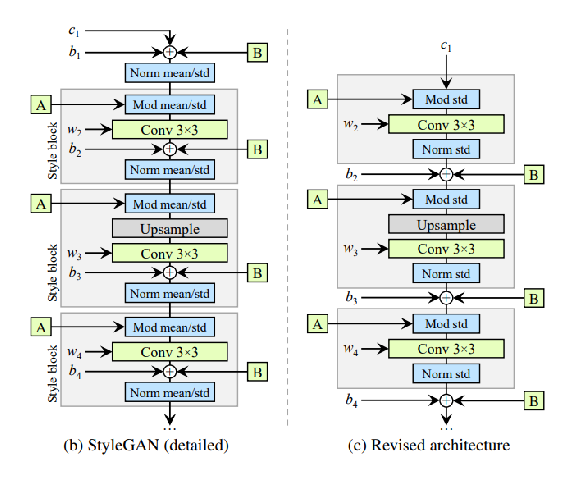
\includegraphics[scale=1.3]{figs/changed-normalization.eps}
    \caption{(b) shows the original StyleGAN architecture. The AdaIN fucntion is shown as combination of normalization and modulation operations. (c) shows the revised model with changes in the network.}\label{Fig:STYLEGAN}
\end{figure}

As seen on the image above, several things changed in the network:

\begin{itemize}
\item Only standard deviation is modified for each feature map, modification of mean was deemed redundant as the effects of this operations were not meaningful for the network. Removing this part made the model simpler,
\item Noise addition was removed from the style block and instead applied inbetween the blocks. This was mainly done to prepare the network for weight modulation,
\item Input vector $c$ is fed to the network directly, without normalization and applying noise.
\end{itemize}

All of these steps were also necessary to introduce the main idea for handling water-droplets artifact problem - \textbf{weight demodulation}.

\begin{figure}[ht!]
    \centering
    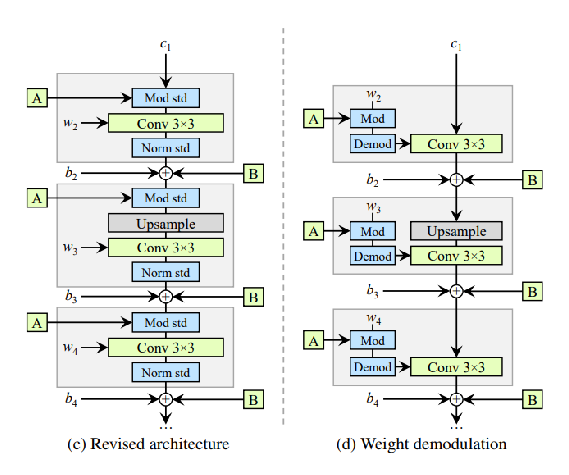
\includegraphics[scale=1.3]{figs/weight-demodulation.eps}
    \caption{(b) shows the original StyleGAN architecture. The AdaIN fucntion is shown as combination of normalization and modulation operations. (c) shows the revised model with changes in the network.}\label{Fig:STYLEGAN}
\end{figure}




% First, have constant input(c) directly as model input rather than modified input C with noise and bias.
% Second, the noise and bias are removed from style block and moved outside.
% At last, we only modify standard deviation per feature map rather than both mean and std.

% The authors of StyleGAN2 explain that this kind of normalization discards information in feature maps encoded in the relative magnitudes of activations. The generator overcomes this restriction by sneaking information past these layers which result in these water-droplet artifacts. The authors share the same confusion as the reader as to why the discriminator is unable to distinguish images from this droplet effect.

% StyleGAN2 like StyleGAN uses a normalization technique to infiltrate styles from W vector using learned transform A into the source imagebut now the droplet artifacts are being taken care of. They introduced Weight Demodulation for this purpose. Let us investigate changes made –

\subsection{Removing Progressive Growing}

StyleGAN2 uses different resolution feature maps that are produced in the base network and uses the ResNet like skip connections to incorporate lower resolutions maps to the final output. This change can be viewed as quite drastic - the whole concept of base network was changed, but it proved to be a necessary step in order to mitigate the \textit{phase artifact} effect.





% StyleGAN2 makes use of the different resolution features maps generated in the architecture and uses skip connections to connect low-res feature maps to final generated image. Bilinear Up/Down-sampling is used within the G and D networks.

% Progressive nature of StyleGAN has attributed to Phase artifacts wherein output images have strong location preference for facial features. StyleGAN2 tries to imbibe the capabilities of progressive growing(training stability for high-res images) and implements a new network design based on skip connection/residual nature like ResNet.

% This new network does not expand to increase image resolution and yet produces the same results. This network is like the MSG-GAN which also uses multiple skip connections. “Multi-Scale Gradients for Generative Adversarial Networks” by Animesh Karnewar and Oliver Wang showcases an interesting way to utilize multiple scale generation with a single end-to-end architecture.

% Main solutions proposed by StyleGAN2

% Eliminating droplet modes by normalizing with estimated statistics instead of AdaIN.
% By using a hierarchical Generator with skip connection (similar to MSG-GAN) instead of Progressive Growing, phase artifacts are reduced.
% Image quality improvement by reducing the Perceptual Path Length (PPL) and smoothing latent space.

% StyleGAN actually generates beautiful and realistic images, but sometimes unnatural parts are generated (artifacts). In the paper "Analyzing and Improving the Image Quality of StyleGAN" these artifacts are exposed and analyzed. Moreover, changes in both model architecture and training methods are proposed to address them.


% We begin by observing that most images generated by
% StyleGAN exhibit characteristic blob-shaped artifacts that
% resemble water droplets. As shown in Figure 1, even when
% the droplet may not be obvious in the final image, it is
% present in the intermediate feature maps of the generator.1
% The anomaly starts to appear around 64×64 resolution,
% is present in all feature maps, and becomes progressively
% stronger at higher resolutions. The existence of such a consistent artifact is puzzling, as the discriminator should be
% able to detect it.
% We pinpoint the problem to the AdaIN operation that
% normalizes the mean and variance of each feature map separately, thereby potentially destroying any information found
% in the magnitudes of the features relative to each other. We



\section{BigGAN}

the BigGAN is a type of conditional GAN utilizing the power of large datasets and huge computational potential. It was proposed by Andrew Brock et al. in 2018 in \cite{biggan}. This architecture is a scaled up version of previous apporaches published by DeepMind team, this time providing larger network and larger batch size. As explained by the authors, this model was trained with two to four times as many parameters as previous networks and with batch size eight times bigger. 

\begin{figure}[H]
    \centering
    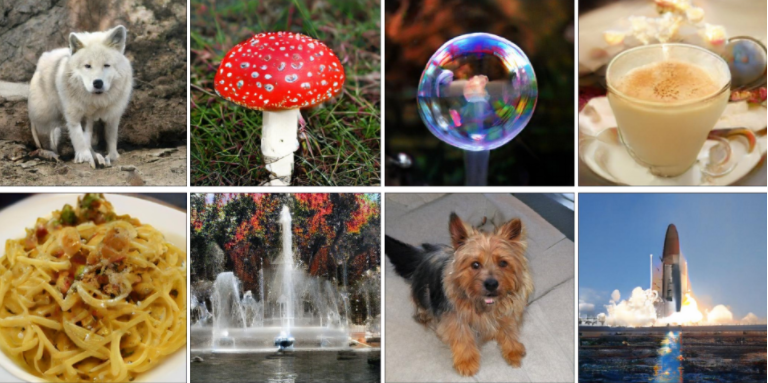
\includegraphics[scale=0.7]{figs/biggan_sample.png}
    \caption{BigGAN examples.}\label{Fig:biggan_sample}
\end{figure}

The largest BigGAN model has over 355 million parameters. The only way of training such huge architecture was to provide ability to train on even 512 Google TPU cores. Final models improved over the previous best IS of 52.52 and FID of 18.65, by achieving IS of 166.3 and FID of 9.6. Additionally, BigGAN also outperformed previous state-of-the-art models at 256x256 and 512x512 resolutions, proving to be a very versatile model.

\begin{figure}[ht!]
    \centering
    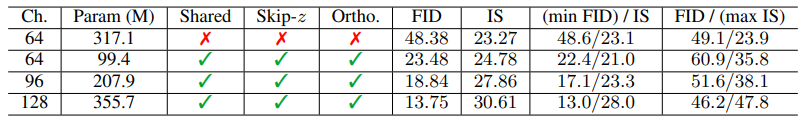
\includegraphics[scale=0.7]{figs/biggan_table.png}
    \caption{BigGAN architecture types with results measured with IS and FID scores.}\label{Fig:biggan_table}
\end{figure}


%The latent vector has a 1-dimensional shape and is usually sampled from a certain probability distribution, where nearby vectors represent similar generated images. BiGans latent vectors are sampled from a truncated normal distribution. The truncated normal distribution is a normal distribution where the values outside the truncation value are resampled to lie again the region inside the truncation region. Here is a simple graph showing truncated normal distribution in the region :

\chapter{Framework description}

\section{Current developments}

\noindent Our work is greatly inspired by current surge of different frameworks and solutions incorporating CLIP model as a mechanism allowing to address several text-to-image problems. As of now, there are several solutions that combine CLIP with generative networks that allow users to retrieve image from the input phrase. Work of Vadim Epstein that can be viewed in \cite{aphantasia} shows high resolution results for abstract image generation using SIREN \cite{siren} and VQGAN \cite{vqgan} neural networks.\

\begin{figure}[H]
    \centering
    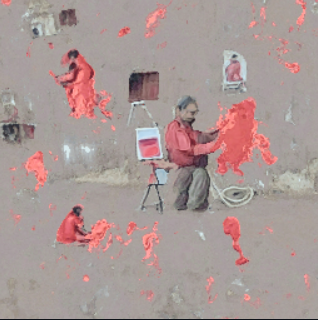
\includegraphics[scale=1.0]{figs/deepdaze.png}
    \caption{Image generated using SIREN \cite{siren} model from "a man painting a completely red image" phrase.}\label{Fig:deepdaze}
\end{figure}

\begin{figure}[H]
    \centering
    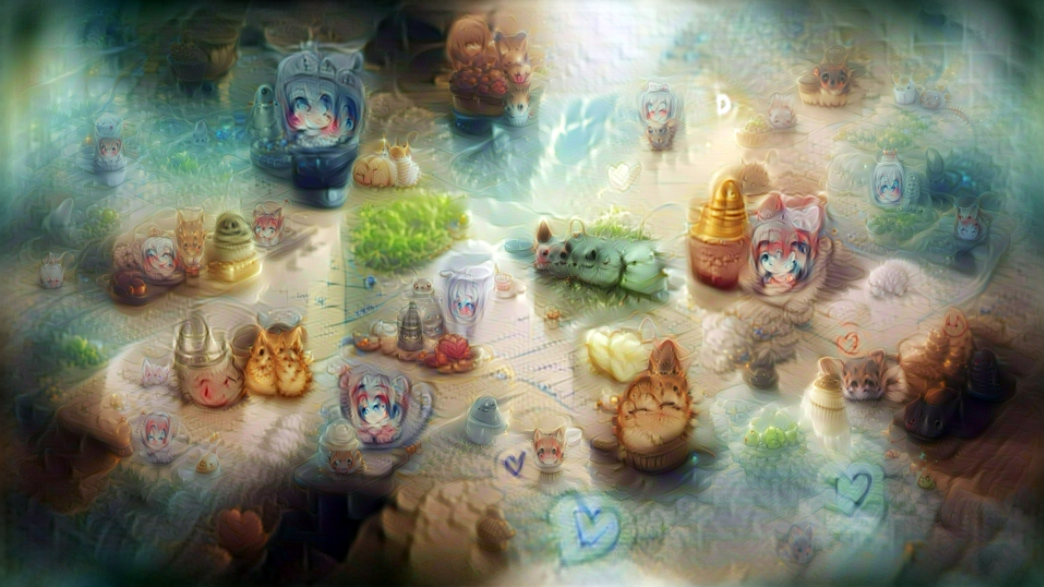
\includegraphics[scale=0.6]{figs/aphantasia.png}
    \caption{Image generated using \textit{Aphantasia} \cite{aphantasia} framework.}\label{Fig:Aphantasia}
\end{figure}

\noindent Approach to latent space searching was explained and researched in \cite{coimbra}. In this paper, authors used genetic algorithm, MAP Elites and random sampling approaches for optimization of fitness function. The results shown there are quite detailed and extensive but presented only for simple GANs trained on MNIST and Fashion MNIST datasets. Authors shown that genetic algorithm was the best performing one from all tested approaches and we decided to capitalize on that result by placing genetic algorithm against differential evolution, which could be a better performing algorithm.

\begin{figure}[H]
    \centering
    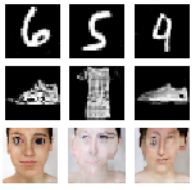
\includegraphics[scale=1.0]{figs/coimbra.png}
    \caption{Random images generated using approach from Fernandes et al. work \cite{coimbra}.}\label{Fig:coimbra}
\end{figure}

\noindent It is worth noticing that many of the current developments related to CLIP models were inspired by Ryan Murdock and Phil Wang and their work on BigGAN latent space exploration, which is titled \textit{Big Sleep} \cite{bigsleep}. Many followers, including us, use similar settings and parameters that allow for extensive image generating based on the BigGAN generator.

%\vspace*{-10mm}

\begin{figure}[H]
    \centering
    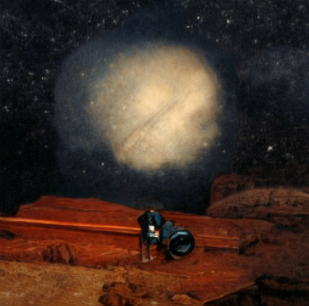
\includegraphics[scale=1.0]{figs/bigsleep.png}
    \caption{Image generated using \textit{Big Sleep} \cite{bigsleep} framework from "the death of the lonesome astronomer" phrase.}\label{Fig:BigSleep}
\end{figure}

%\vspace*{-10mm}

\noindent There are several APIs dedicated for text-to-image generation that can be found, but all of them show very low generative capabilities, which accurately reflects current state of matter in this domain.

\begin{figure}[H]
    \centering
    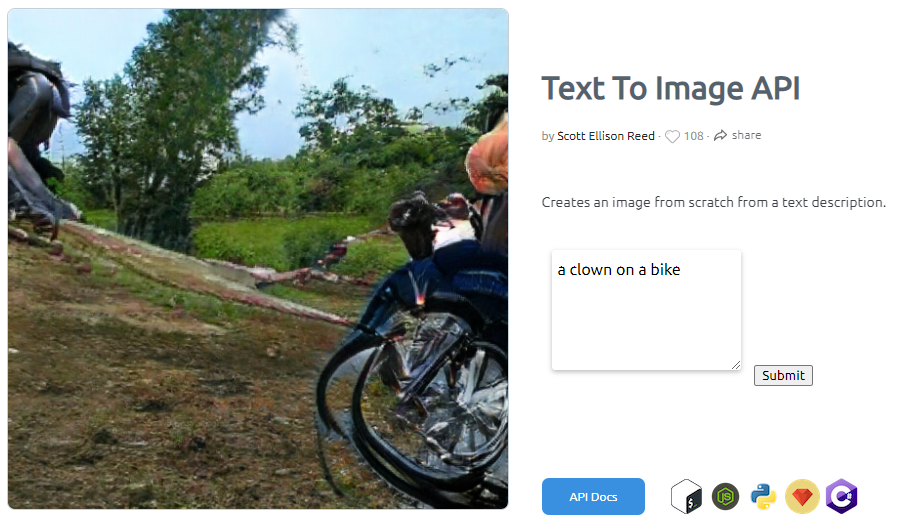
\includegraphics[scale=0.6]{figs/deepai.png}
    \caption{Image generated using \textit{DeepAI} \cite{deepai} text-to-image API from "a clown on a bike" phrase.}\label{Fig:deepai}
\end{figure}

\section{Overview}

The architecture of solution that we are exploring in this work consists of four main components:
\begin{enumerate}
\item Pre-trained generative model based on Generative Adversarial Network architecture,
\item CLIP model,
\item Evolutionary optimization algorithm,
\item Evaluation using classification network.
\end{enumerate}
Graph below shows the flow of data and describes the overall framework architecture:\\


\begin{figure}[H]
    \centering
    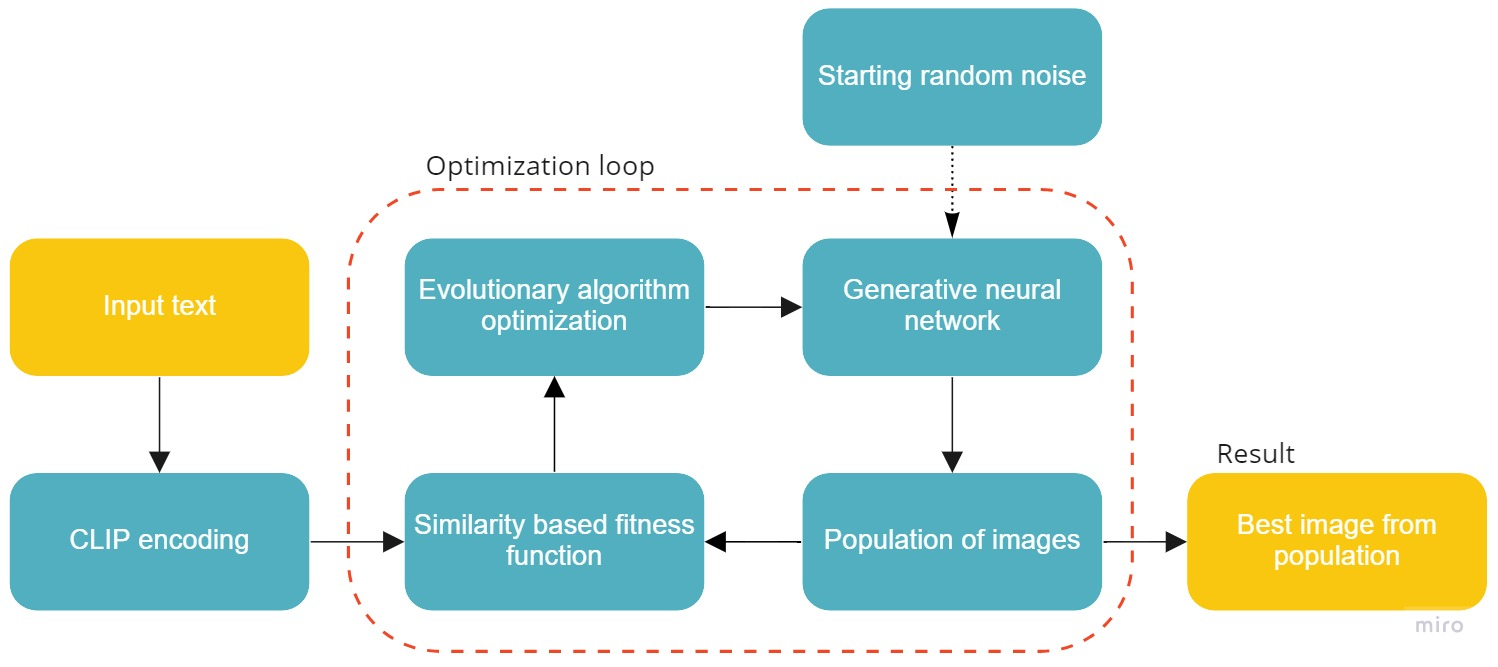
\includegraphics[scale=0.6]{figs/flow.png}
    \caption{Flowchart presenting the entire process of generating an image from text.}\label{Fig:flow}
\end{figure}

\noindent Description of the flowchart:
\begin{enumerate}
\item [1.] First, text is provided by the user,
\item [2.] Introduced text is encoded using pre-trained CLIP model.
\end{enumerate}
Next steps can be considered as a 'optimization loop':
\begin{enumerate}
\item [3a.] Algorithm is performing optimization step,
\item [3b.] Optimized population of samples (vectors)  is serving as an input for generator which produces images,
\item [3c.] Generated images are evaluated by fitness function (in our case, similarity function).
\end{enumerate}
After completing this process, post-processing part takes place:
\begin{enumerate}
\item [4.] Output images are passed for an evaluation using classification network and similarity metric.
\end{enumerate}

We consider StyleGAN2 and BigGAN architectures as the main choice for a generative models in this solution. Main advantages of that choice are:
\begin{itemize}
\item These are widely available as a pre-trained structures; StyleGAN2 is public and open-sourced for both generative and discriminative parts of the architecture, BigGAN is public as a generative part of the model. 
\item StyleGAN2 consists of several class-based dedicated models (such as StyleGAN2-car or StyleGAN2-ffhq). It allows for experimentations with different types of images and checking the experiments results between both type of GANs.
\item Both of these models are still considered to be state-of-the-art regarding the quality of produced images and were trained using huge datasets of images. This leads to much more interesting and explorable results.
\end{itemize}

\noindent We decided to use two algorithms described in previous chapters - \textit{genetic algorithm} and \textit{differential evolution}. First one was already tested to some extend in previous works (\cite{coimbra}). Latter one is considered to be an upgraded version and is regarded to converge quicker and provide more stable results. We decided to test how well these two can perform against each other when providing same hyperparameters.

\noindent Implementation wise, we decided to use the boilerplates for these algorithms provided by the \textit{pymoo} library. We performed some changes in the source code in order to fully match our needs for experiments. We also made sure that the experiments coded in the library and used as API were correctly implemented and matching with definitions we provided in the theory section of this work. Using some high-level functions from this library allowed us to generate results much quicker than it would have been when defining functions by hand from the scratch.

\noindent Finally, we managed to migrate the code from the general repository to the Google Colab based environment. It allows any user to generate own images in the scope of models and algorithms that are implemented. User can choose several generation options, such as the number of generations, how often outputs should be viewed etc.

\begin{figure}[H]
    \centering
    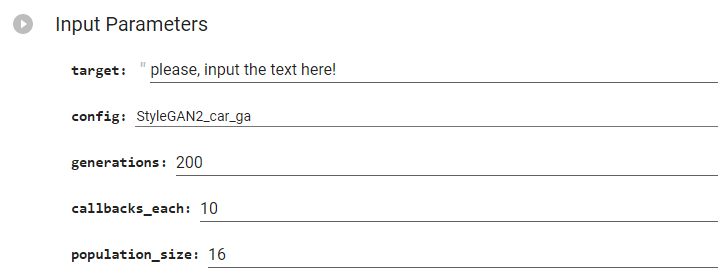
\includegraphics[scale=0.8]{figs/collab.png}
    \caption{Google Colab cell presenting possible settings for image generation.}\label{Fig:collab}
\end{figure}


\chapter{Experiments}

\section{Examples and observations}

\noindent By using the framework we were able to obtain objectively good quality images for different phrases. Given enough time (large enough number of generations) the algorithm is able to guide generator into the correct region of latent space. Using dedicated StyleGAN2 models by providing the text description from the area of training showed some well adjusted results.

\begin{figure}[H]
    \centering
    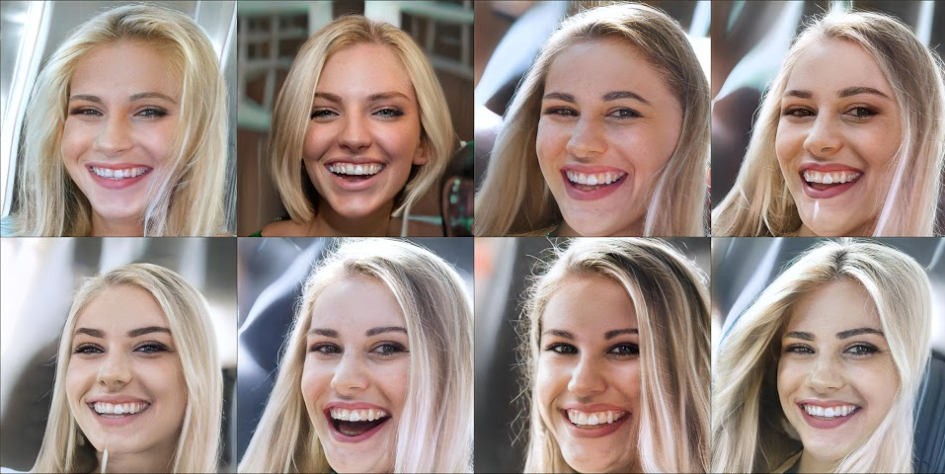
\includegraphics[scale=0.6]{figs/blondgirl.png}
    \caption{Images generated with GA and StyleGAN2-ffhq model with the "a blond girl with a smile" phrase.}\label{Fig:blondgirl}
\end{figure}

\noindent Using BigGAN model also proved successful, especially in terms of general usage and for the phrases that were not manageable by the dedicated StyleGAN2 models.

\begin{figure}[H]
    \centering
    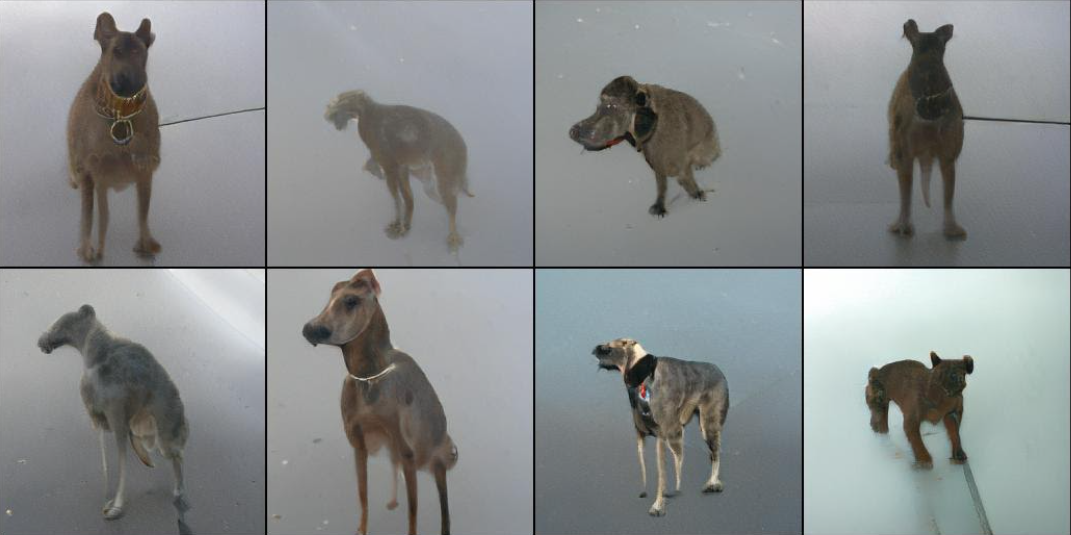
\includegraphics[scale=0.55]{figs/doginthefog.png}
    \caption{Images generated with GA and BigGAN model with the "a dog in the fog" phrase.}\label{Fig:doginthefog}
\end{figure}

\noindent Differences between two models will be discussed later in the work.\newline
\noindent The general rules of evolutionary algorithms, mainly the fact that they are based on population calibration, are visible in many results of conducted experiments. On of the main observations is that when launched for long enough, all of the images in the last populations are looking very similar. That could be perceived as equivalent of \textit{overtraining} the neural network - by prolonging the process we lose the variety of generated images and are left with very alike pictures.

\begin{figure}[H]
    \centering
    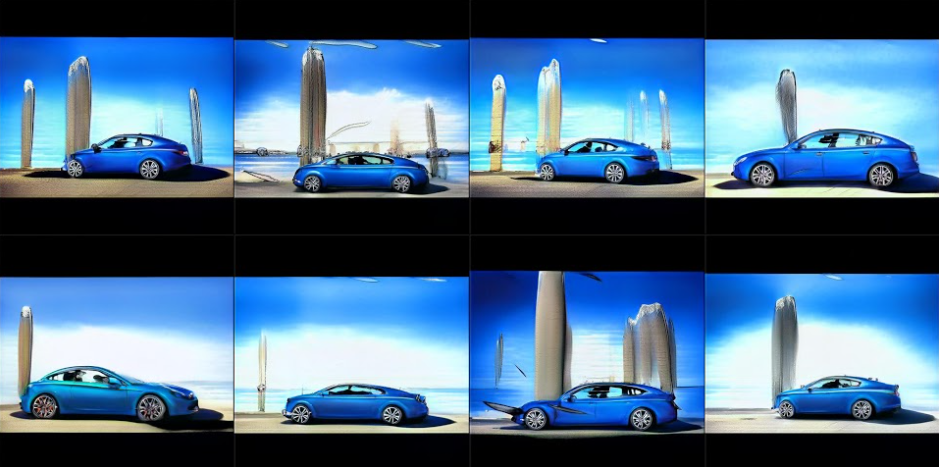
\includegraphics[scale=0.6]{figs/bluecar.png}
    \caption{Images generated with GA and StyleGAN2-car model with the "a blue car near the water in sun" phrase.}\label{Fig:bluecar}
\end{figure}

\subsection*{Cosine similarity analysis}
\noindent One of the aspects we decided to analyze is the behavior of cosine similarity values in the context of our model. This function is used mainly in two aspects of the work:
\begin{itemize}
\item  as a loss function in CLIP model,
\item as a fitness function for evolutionary algorithms.
\end{itemize}
\noindent The most important application of cosine similarity seems to be the ability to determine how similar according to the model the input phrase and the generated image are.  We performed several experiments in order to verify the range of values that the model is producing.

\begin{figure}[H]
\centering
\begin{subfigure}[b]{1\textwidth}
\centering
   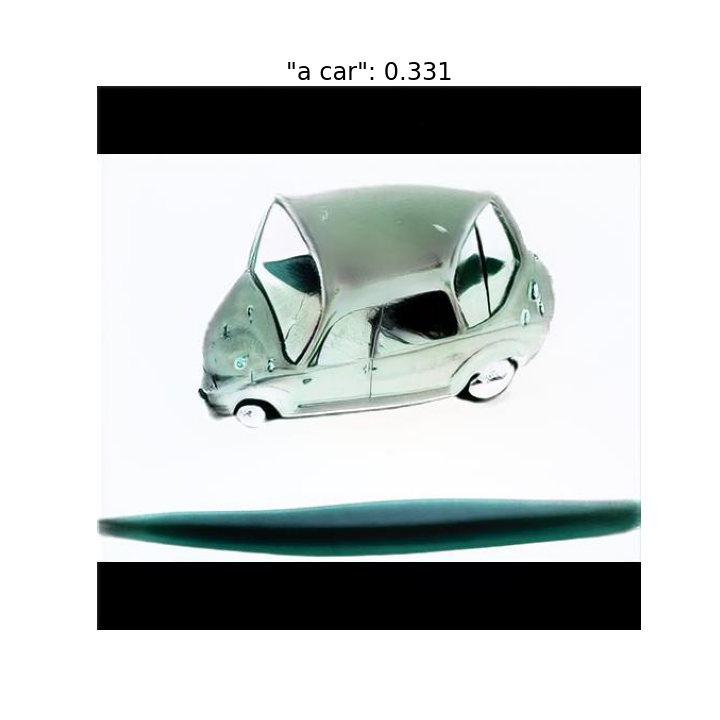
\includegraphics[width=0.5\linewidth]{figs/a car_cossim.png}
\end{subfigure}

\begin{subfigure}[b]{1\textwidth}
\centering
   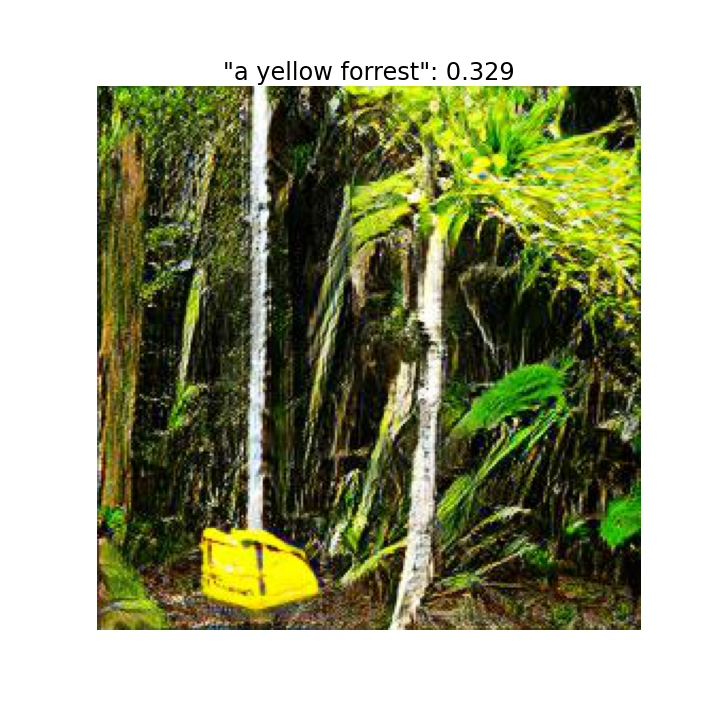
\includegraphics[width=0.5\linewidth]{a yellow forrest_cossim.png}
\end{subfigure}

\begin{subfigure}[b]{1\textwidth}
\centering
   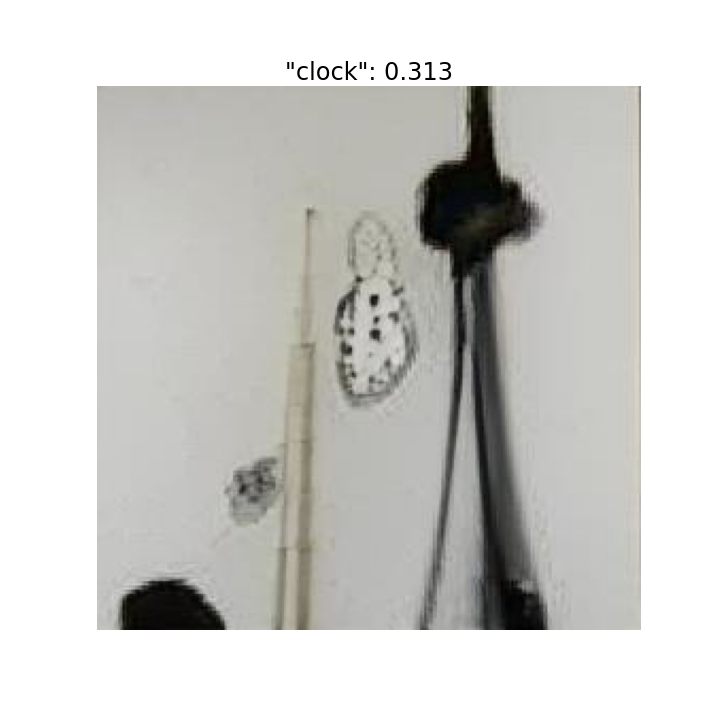
\includegraphics[width=0.5\linewidth]{clock_cossim.png}
\end{subfigure}

\end{figure}

\noindent Based on the above examples (as well as other tests performed during the research), we noticed that the values in our solution usually oscillate in the range of $0.2 - 0.4$. We see that even in obvious cases, such as the phrase "a car", after long enough generation the value reaches plateau of $0.331$.  \\
\noindent We observed similar behavior during our research on CLIP model - many users before us noticed such regularity in their tests.
Although it seems that cosine similarity, which we determine for a pair of image-query in our solution, cannot be interpreted for a single image, we noticed from our work on evolutionary algorithms that it may be used as a metric comparing different images generated for the same query. Let us look at the following examples:
\begin{figure}[H]
    \centering
    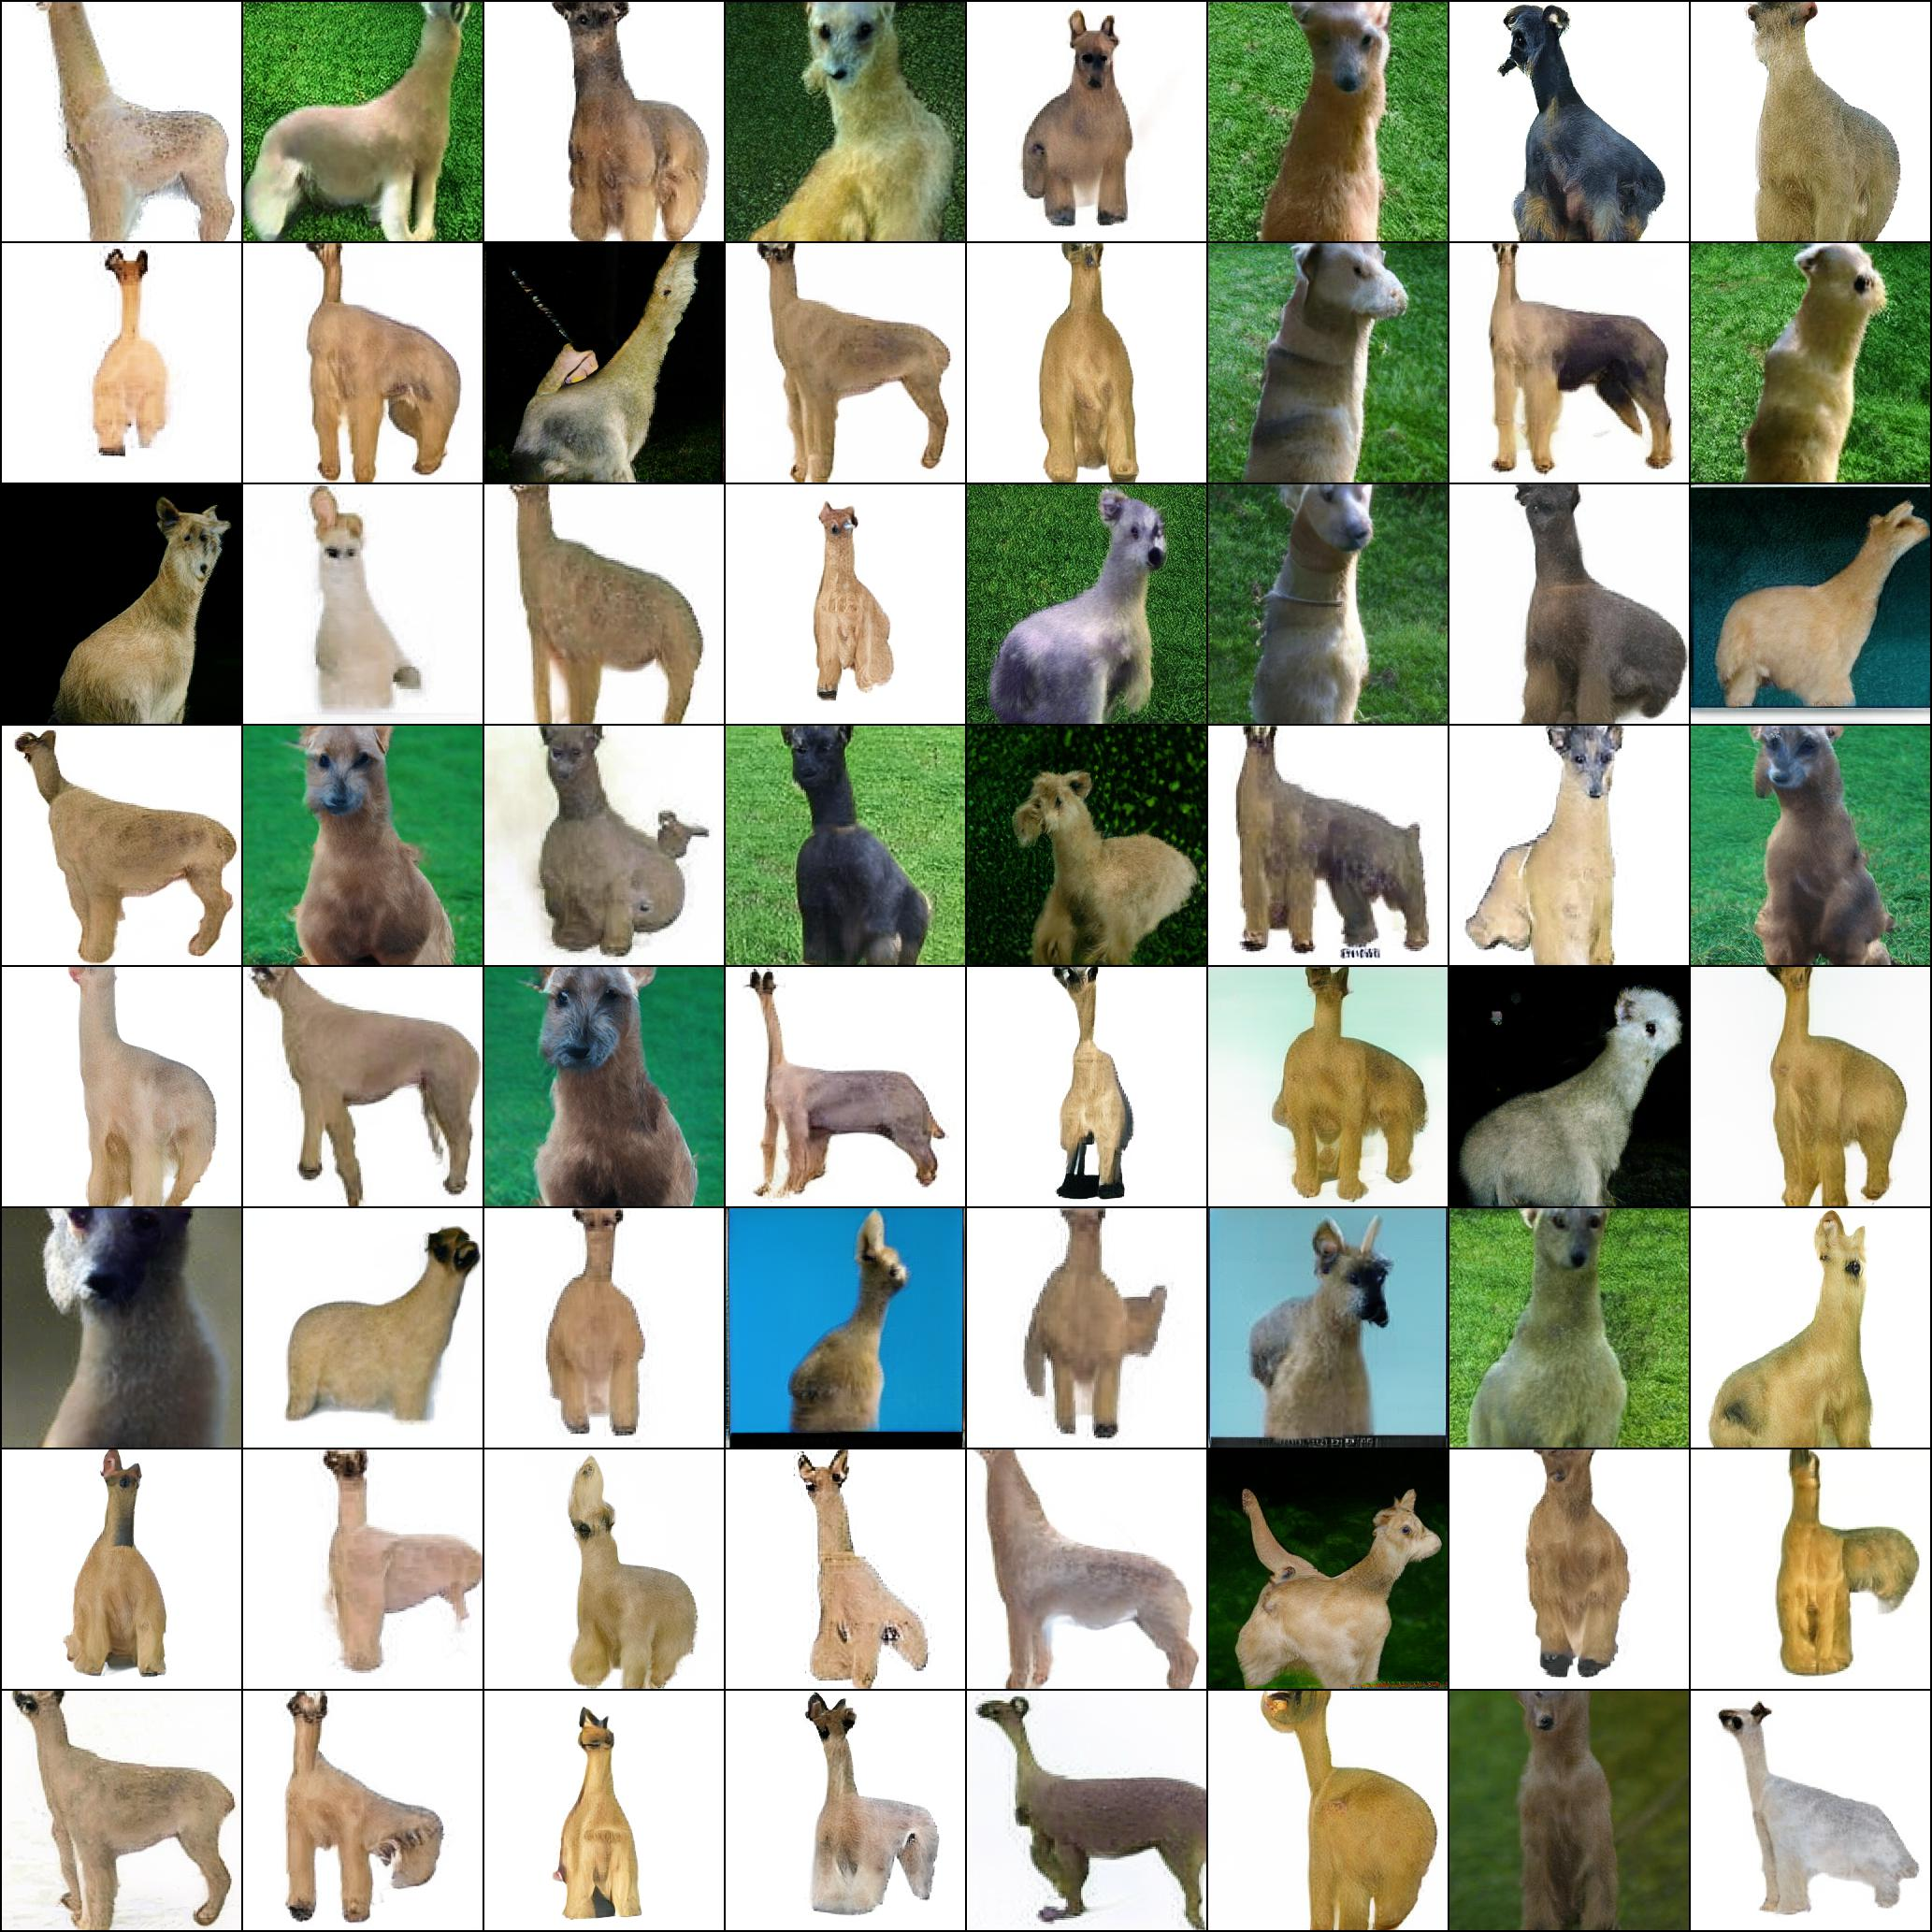
\includegraphics[scale=0.2]{figs/batch_loop_7.jpg}
\end{figure}
\noindent The generation from the genetic algorithm for \textit{llama} input phrase,  sorted by \textit{cos-sim} from the top left corner - we can see that the further away the photo deviates slightly more from the given phrase. \\
\begin{figure}[H]
    \centering
    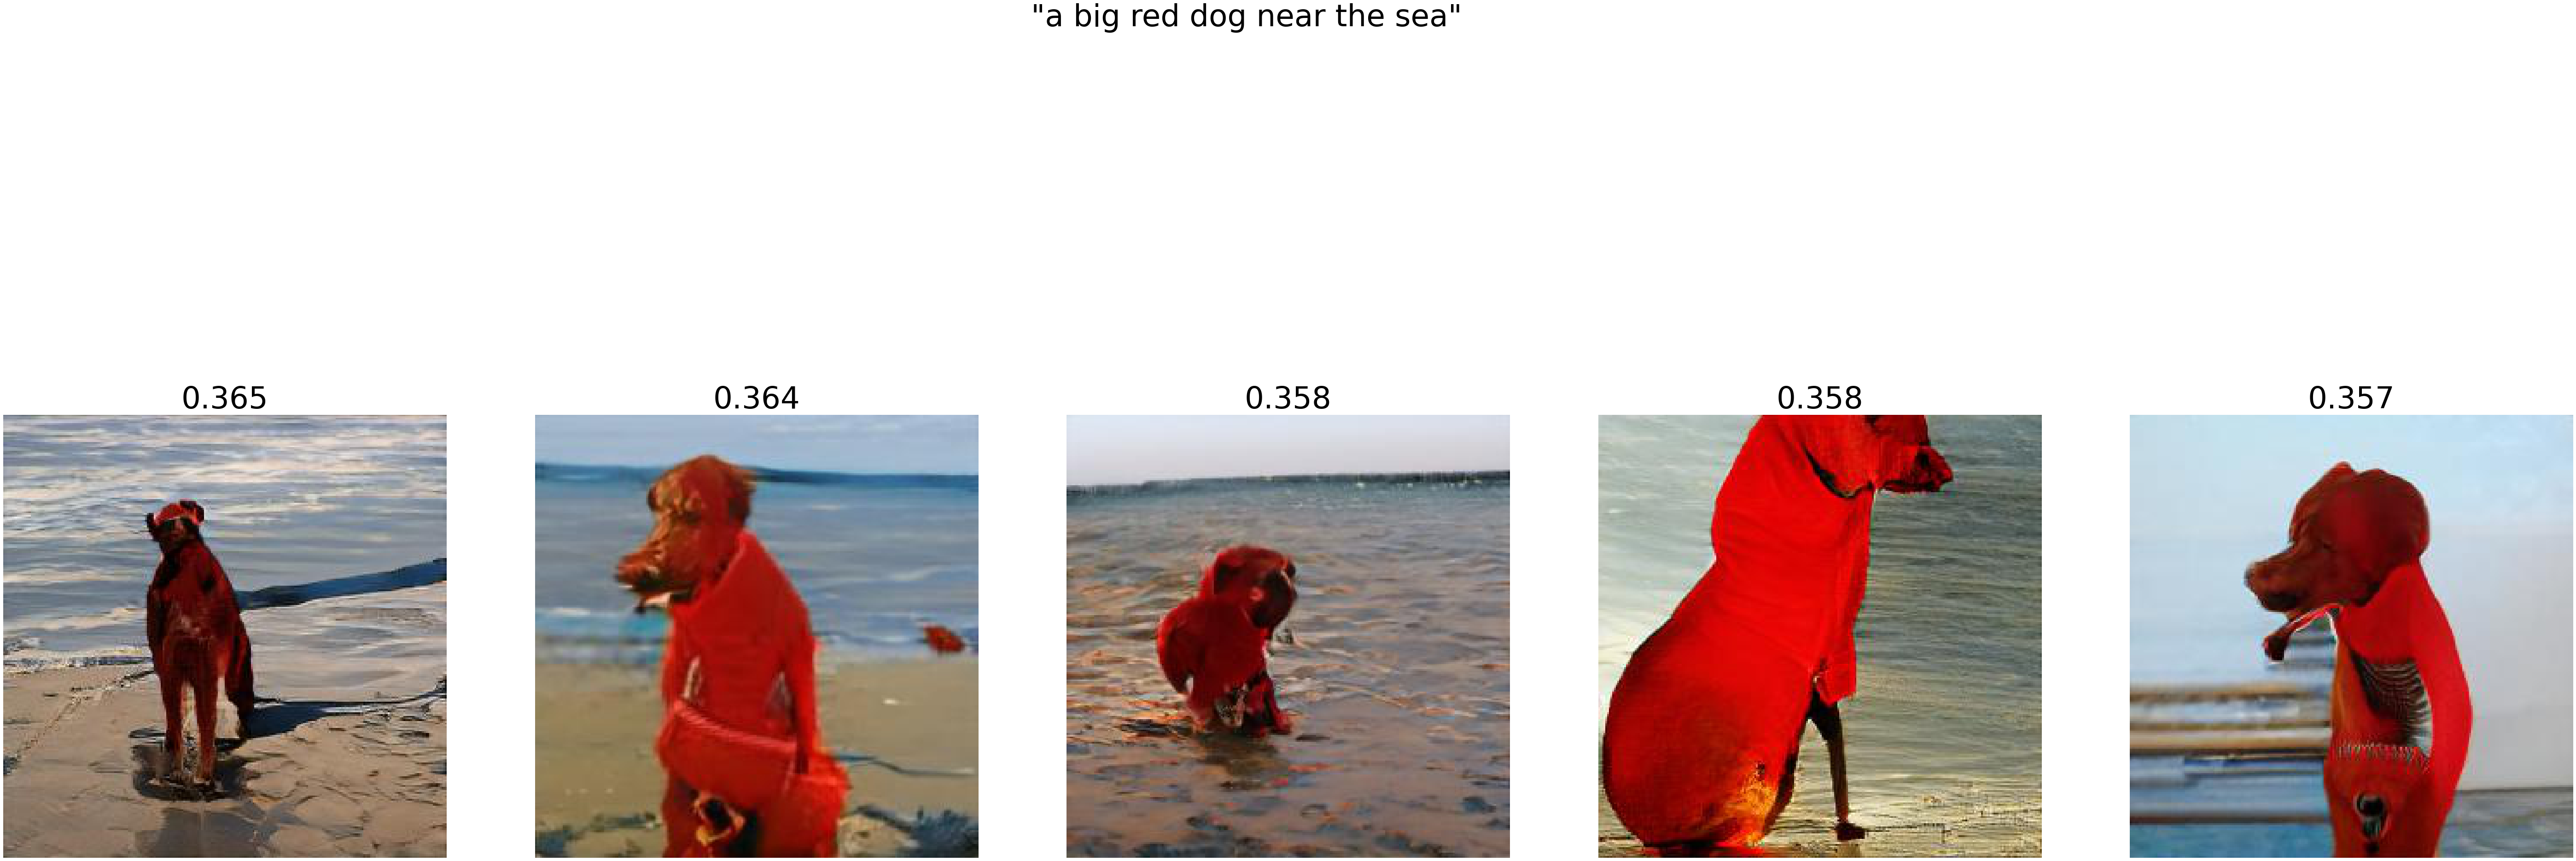
\includegraphics[scale=0.08]{figs/bigreddog.png}
\end{figure}
\noindent Five images generated as results of the genetic algorithm we have implemented. We can see that values differ only on decimal places, but images with higher value are slightly better reflecting given phrase.\\

\section{Genetic Algorithm vs Differential Evolution}

Both of the algorithms presented in this work are population based and work applying similar techniques and concepts. Even though, by testing different scenarios we noticed that several patterns emerged for the generating process using both of these algorithms. 
Differential evolution algorithm starts converging slower than genetic algorithm. It is especially visible in the first generations of the algorithms e.g. 10th generation. Images produced by generator after steering with genetic algorithm tend to be visually (and according to the metric) closer to the target text. First figure below shows this occurrence.\\
The input phrase used to generate was '\textit{\textbf{a yellow car in the city}}'. Dedicated model trained on car images was used - StyleGAN2-car. Population obtained from genetic algorithm after 10 generations already has some acceptable units based on the input phrase. Cars are yellow (some of them deformed but the color is correct) and some of them are in the urban space. That means that genetic algorithm already steered the latent vector into the embedding of information about yellow color, car and the city.\\
On the other hand, differential evolution did not process the information about color yet - produced cars are random in that subject.

\newpage

\begin{figure}[H]
\centering
\begin{subfigure}[b]{1.0\textwidth}
   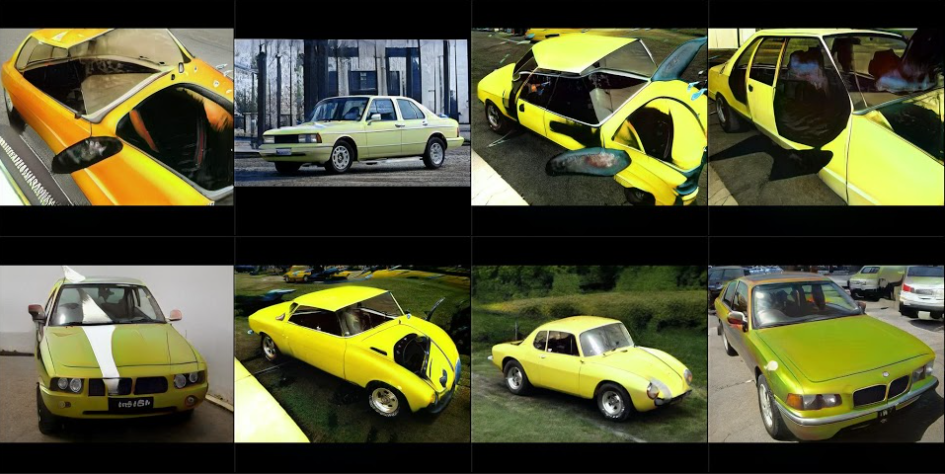
\includegraphics[width=1\linewidth]{GA_yellowcar_10.PNG}
   \caption{genetic algorithm}
   \label{fig:Ng1} 
\end{subfigure}

\begin{subfigure}[b]{1.0\textwidth}
   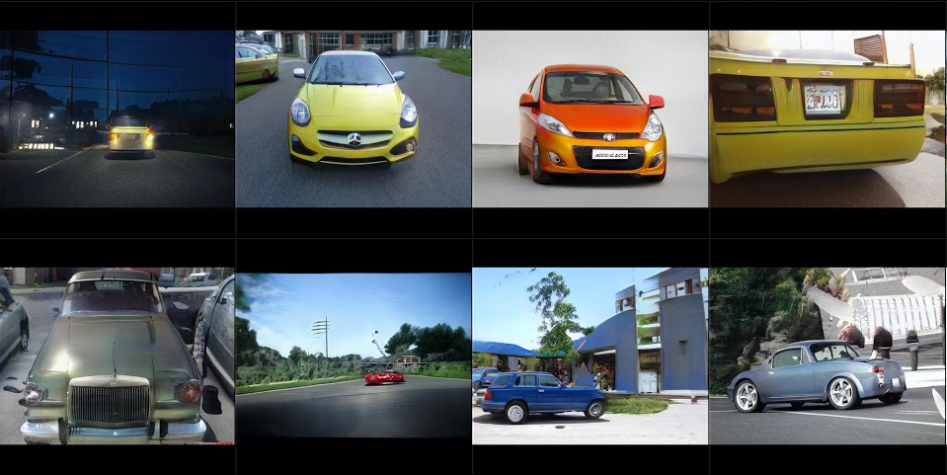
\includegraphics[width=1\linewidth]{DE_yellowcar_10.PNG}
   \caption{differential evolution}
   \label{fig:Ng2}
\end{subfigure}

\caption[Two numerical solutions]{10th generation of evolutionary algorithms traversing the latent space.}
\end{figure}

\newpage

\begin{figure}[H]
\centering
\begin{subfigure}[b]{1.0\textwidth}
   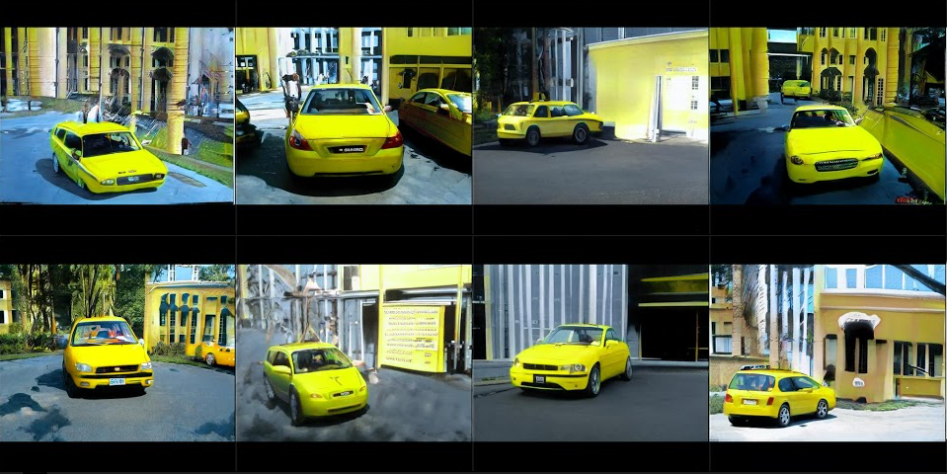
\includegraphics[width=1\linewidth]{GA_yellowcar_100.PNG}
   \caption{genetic algorithm}
   \label{fig:Ng1} 
\end{subfigure}

\begin{subfigure}[b]{1.0\textwidth}
   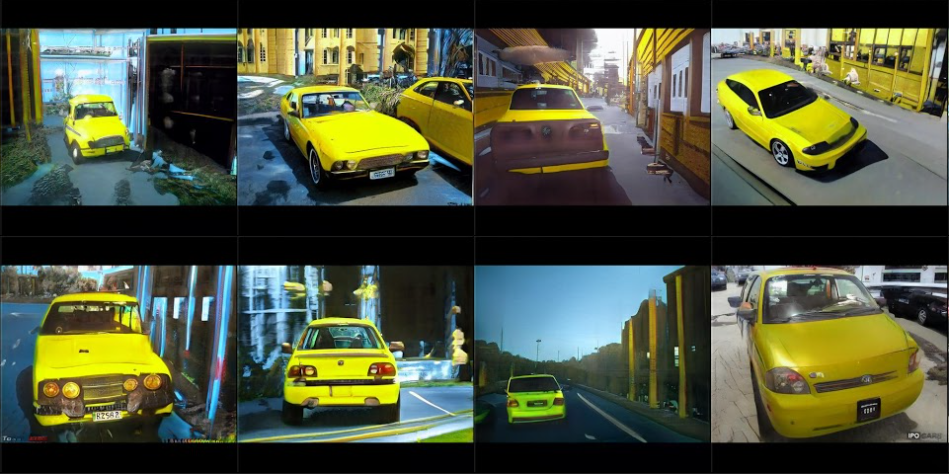
\includegraphics[width=1\linewidth]{DE_yellowcar_100.PNG}
   \caption{differential evolution}
   \label{fig:Ng2}
\end{subfigure}

\caption[Two numerical solutions]{100th generation of evolutionary algorithms traversing the latent space.}
\end{figure}

\newpage

\begin{figure}[H]
\centering
\begin{subfigure}[b]{1.0\textwidth}
   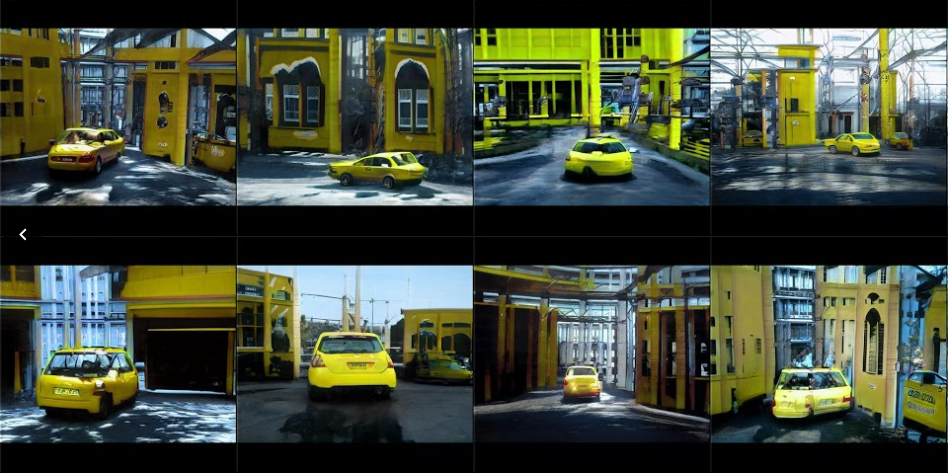
\includegraphics[width=1\linewidth]{GA_yellowcar_200.PNG}
   \caption{genetic algorithm}
   \label{fig:Ng1} 
\end{subfigure}

\begin{subfigure}[b]{1.0\textwidth}
   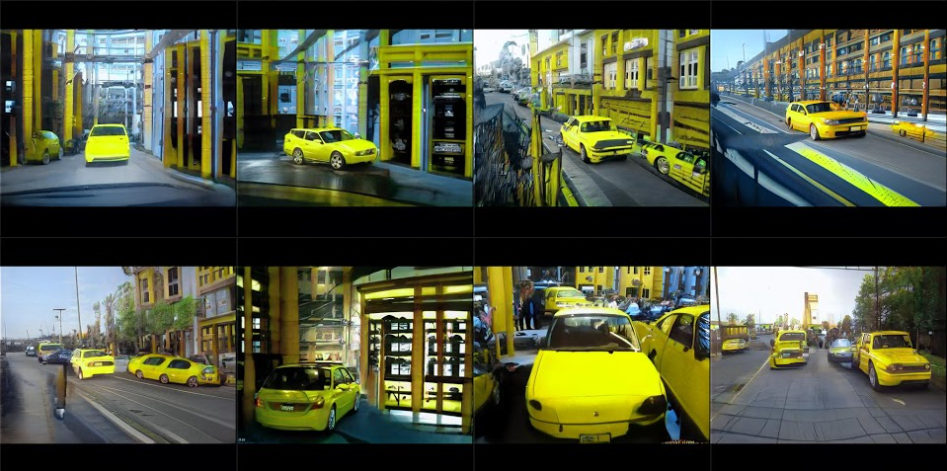
\includegraphics[width=1\linewidth]{DE_yellowcar_200.PNG}
   \caption{differential evolution}
   \label{fig:Ng2}
\end{subfigure}

\caption[Two numerical solutions]{200th generation of evolutionary algorithms traversing the latent space.}
\end{figure}

Interestingly, we can notice that model is not comprehending the input phrase with the human-like ability - one of the examples would be 'leaking' of the context in the phrase. For instance, images from the final generation (from both algorithms) of the phrase 'a yellow car in the city' are visibly containing a lot of yellow color beside the color of the car. From human perspective, background and surroundings of the yellow car should remain arbitrary in terms of color, since only the car is supposed to be yellow according to the phrase. Generator is feeling more confident about the produced image when yellow color is cascaded on the buildings and objects around the car. Moreover, this type of model behaviour is amplified when bright colors are used in the input phrase (such as yellow, light green).

\begin{figure}[H]
    \centering
    \includegraphics[scale=0.45]{figs/avg_mean.jpg}
    \caption{Plot of the mean reversed cosine similarity values for generations from 0 to 200 for 50 consecutive runs. Orange line presents differential algorithm while blue line shows genetic algorithm.}\label{Fig:STYLEGAN}
\end{figure}

\begin{figure}[H]
    \centering
    \subfloat[\centering genetic algorithm]{{\includegraphics[width=7cm]{GA_yellowcar_final.PNG} }}%
    \qquad
    \subfloat[\centering differential evolution]{{\includegraphics[width=7cm]{DE_yellowcar_final.PNG} }}%
    \caption{Final images produced by algorithms.}%
    \label{fig:example}%
\end{figure}

\noindent One of the benefits and features of using a population based algorithm for image generating is the fact that many 'similar' in terms of quality pictures are produced. The final images taken from the model have certain visible flaws - the city seems to be rendered in acceptable manner but the cars are somewhat deformed. The good part of using whole population as the output of the model is that a human can objectively choose the best image from the last produced generation. It is vital given the fact, that last images are usually close to each other in terms of scoring (which means that choosing the single final image is not based on strong decision making) but present vastly different scenarios for the input phrase.\\

\noindent Below is one more plot, showing the dynamics of change in the lowest fitness values for both algorithms in every algorithm population.

\begin{figure}[H]
    \centering
    \includegraphics[scale=0.45]{figs/best_both.jpg}
    \caption{Plot of the best sample values for each population for the "a yellow car in the city" phrase and both algorithms.}\label{Fig:STYLEGAN}
\end{figure}

\section{StyleGAN2 vs BigGAN}

\noindent It is apparent that the underlying dataset is crucial in determining the generative power of the model. Throughout the experiments, we noticed that there are two separate use cases for both StyleGAN2 and BigGAN models. 

\noindent First, we observed that StyleGAN2 is outperforming BigGAN model significantly when user provides a phrase that is related to the dataset that the model was trained on. Even though this conclusion might seem obvious, we still found the results from both models interesting.

\begin{figure}[H]
\centering
\begin{subfigure}[b]{1.0\textwidth}
   \includegraphics[width=1\linewidth]{redgothic_stylegan.PNG}
   \caption{StyleGAN2-church}
   \label{fig:Ng1} 
\end{subfigure}

\begin{subfigure}[b]{1.0\textwidth}
   \includegraphics[width=1\linewidth]{redgothic_biggan.PNG}
   \caption{BigGAN}
   \label{fig:Ng2}
\end{subfigure}
\caption[pics]{Comparison of StyleGAN2-church and BigGAN models for a "red gothic church" phrase.}
\end{figure}

\noindent As we can see on above example, the BigGAN model has the idea about the color, but the general church object is not properly embedded in latent space, hence the model tries to generate some structures that it identifies as 'gothic'. Similar inaccuracies are visible in the next example also.

\begin{figure}[H]
\centering
\begin{subfigure}[b]{1.0\textwidth}
   \includegraphics[width=1\linewidth]{gingerboy_stylegan.PNG}
   \caption{StyleGAN2-ffhq}
   \label{fig:Ng1} 
\end{subfigure}

\begin{subfigure}[b]{1.0\textwidth}
   \includegraphics[width=1\linewidth]{gingerboy_biggan.PNG}
   \caption{BigGAN}
   \label{fig:Ng2}
\end{subfigure}
\caption[pics]{Comparison of StyleGAN2-ffhq and BigGAN models for "a ginger boy" phrase.}
\end{figure}

\noindent Again, we can see clear outputs produced by the StyleGAN2 model, while images produces by BigGAN are fairly deformed and not representative. On the other hand, we can see that again BigGAN tried to transfer information about color to the picture - hence every \textit{person} on an image has red shirt.\\

\noindent On the other hand, in every other aspect, BigGAN is able to generalize better and find more appropriate representation of input text than StyleGAN. Once again, it is a direct implication of the dataset that both models were trained with. 

\begin{figure}[H]
\centering
\begin{subfigure}[b]{1.0\textwidth}
   \includegraphics[width=1\linewidth]{clown_stylegancat2.PNG}
   \caption{StyleGAN2-cat}
   \label{fig:Ng1} 
\end{subfigure}

\begin{subfigure}[b]{1.0\textwidth}
   \includegraphics[width=1\linewidth]{clown_stylegancar.PNG}
   \caption{StyleGAN2-car}
   \label{fig:Ng2}
\end{subfigure}

\caption[pics]{Comparison of StyleGAN2-cat and StyleGAN2-car for "a clown cyclist on the moon" phrase.}
\end{figure}


\noindent StyleGAN2 models output can be described as close to randomize - model is trying to generate a meaningful image while having no idea about \textit{the moon}, \textit{clown} and \textit{cyclist}. This results in a random walk through the latent space and provides images which are not making much sense. With this example, we can clearly see the advantage of the BigGAN model - images from the last population clearly show the moon-like surface, elements of clown's hat and circus stadium as well as machines that resemble a bike.

\begin{figure}[H]
    \centering
    \includegraphics[scale=0.55]{figs/clown_biggan.PNG}
    \caption{BigGAN model ouput for "a clown cyclist on the moon" phrase.}\label{Fig:clownbiggan}
\end{figure}

\noindent Provided examples show the power of data and datasets used for training. Having enough data there could be a possibility of creating a model combining the best of two worlds from StyleGAN2 and BigGAN - a model that is producing crips images with high quality (like dedicated StyleGAN2) and also has a wide variety of generative possibilities (like BigGAN).

\newpage

\chapter{Evaluation}

%https://www.cs.toronto.edu/~kriz/cifar.html

\noindent In order to evaluate the model we described, we decided to see if the images we generated would be able to \textit{fool} the classifiers learned on popular datasets.
We took two famous and widely used datasets as our benchmarks.
\subsection*{CIFAR10}
\noindent CIFAR-10 dataset consists of 60000 32x32 color images in 10 classes, with 6000 images per class. There are 50000 training images and 10000 test images. The classes are mutually exclusive. Below are the classes in the dataset, as well as 10 random images from each:
\begin{figure}[H]
    \centering
    \includegraphics[scale=0.6]{figs/cifar10_dataset.png}
    \caption{Examples from CIFAR10 dataset. \cite{cifar10_data}.}
\end{figure}
\noindent CIFAR10 dataset can be downloaded from \cite{cifar10_data}.
\subsection*{ImageNet} 
\noindent ImageNet dataset contains 14 197 122 hand-annotated images. Since 2010 the dataset is used in the ImageNet Large Scale Visual Recognition Challenge (ILSVRC), a benchmark in image classification and object detection.  ImageNet contains more than 20000 categories. This dataset is especially useful in many evaluation cases because it contains general groups of objects (such as \textit{balloon} or \textit{strawberry}) as well as detailed categories e.g. dogs' breeds names like \textit{rottweiler} or \textit{Old English sheepdog}.
\begin{figure}[H]
    \centering
    \includegraphics[scale=0.5]{figs/imagenet.png}
    \caption{Examples from ImageNet dataset \cite{imagenet_example}.}
\end{figure}
\noindent Dataset can be downloaded from \cite{imagenet_data}. \\
\noindent Having selected datasets, we chose classifiers trained on them with high accuracy scores:\\
\begin{itemize}
\item CIFAR-10 CNN Classifier \cite{cifar10_classifier} - with $ \sim 85\% $ accuracy.
\item ImageNet - ResNet-50 Classifier \cite{resnet} -  with $ \sim 76\% $ accuracy. 
\end{itemize}

\noindent For evaluation purposes, we generated fixed number of images for selected classes from both datasets (based on the class names), and then reported what accuracy they achieved when passed through the corresponding classifiers. \\
\noindent For the CIFAR10 dataset we will generate images for each of the 10 available classes: \\
\noindent \textbf{[airplane, automobile, bird, cat, deer, dog, frog, horse, ship, truck]}.\\
For the ImageNet dataset, we chose 10 classes each of them coming from different domain for variety purposes: \\
\noindent \textbf{[llama,  cash machine,  hammer,  miniskirt,  pirate,  shopping cart,  wall clock,  ice cream,  banana, Kerry blue terrier]} 
\newline
Both evaluations were performed using intentionally selected model, algorithm and parameters settings:
\begin{itemize}
\item GAN model used - \textbf{DeepMindBigGAN256}
\item Evolutionary model used - \textbf{GA}
\item Population size - $\bm{64}$
\item Number of model repetitions - $\bm{8}$
\item Number of images generated per class - $\bm{512} = 512 = 64$
\end{itemize}

\section{CIFAR10}
\noindent We present results of our evaluation in the form of the following table. \\
\begin{table}[h!]
\centering
\begin{tabular}{|l|c|c|c|}
\hline
\multicolumn{1}{|c|}{\textbf{Class}} & \textbf{Positive} & \textbf{Negative} & \textbf{Accuracy (\%)}       \\ \hline
AIRPLANE                             & 476               & 36                & {\color[HTML]{32CB00} 92.97} \\ \hline
AUTOMOBILE                           & 88                & 424               & 17.19                        \\ \hline
BIRD                                 & 12                & 500               & 2.34                         \\ \hline
CAT                                  & 177               & 335               & 34.57                        \\ \hline
DEER                                 & 0                 & 512               & {\color[HTML]{FE0000} 0.0}   \\ \hline
DOG                                  & 255               & 257               & 49.8                         \\ \hline
FROG                                 & 39                & 473               & 7.62                         \\ \hline
HORSE                                & 64                & 448               & 12.5                         \\ \hline
SHIP                                 & 60                & 452               & 11.72                        \\ \hline
TRUCK                                & 97                & 415               & 18.95                        \\ \hline
\textbf{TOTAL}                       & \textbf{1268}     & \textbf{3852}     & \textbf{24.77}               \\ \hline
\end{tabular}
\end{table}
\newline
\noindent The \textit{positive} column informs about the number of images generated by the model that were classified correctly, and \textit{negative} column yields the number of incorrectly classified images. From the summary of the experiment we notice that almost $25\%$ of images generated by the model were classified correctly across all 10 classes. For this type of dataset, it is more informative to look at the results on the class basis.
\noindent For most of the classes the accuracy is way below $50\%$. Model had most difficulties with classes like \textit{deer}, \textit{bird} and \textit{frog}. On the other side, \textit{airplane} class had a very large score $90\%$.\\

\noindent \textbf{Airplane}
\begin{figure}[ht!]
    \centering
    \includegraphics[scale=0.45]{figs/cifar10_examples/airplane.png}
\end{figure} 
\newline
\noindent We see that the generated images of the \textit{airplane} mostly show its wing against the sky. We can surmise that the classifier was right so often on the \textit{airplane} images we generated, because they included the blue sky.
\newpage
\noindent \textbf{Dog} \\
\begin{figure}[ht!]
    \centering
    \includegraphics[scale=0.45]{figs/cifar10_examples/dog.png}
\end{figure}
\newline It's hard to see a feature that distinguishes correctly and incorrectly classified images in the \textit{dog} class. Instead, it can be seen that the \textit{dog} images generated by the model are quite readable. Later in the chapter we will look at what other classes this class was confused with.
\newline
\newline
\noindent \textbf{Deer} \\
\begin{figure}[ht!]
    \centering
    \includegraphics[scale=0.45]{figs/cifar10_examples/deer.png}
\end{figure}
\newline 
\noindent \textit{Deer} class was not even once classified correctly. We can see that the generated \textit{deers} resemble \textit{dogs} with some element that may represent antlers. We suspect that the model failed this task because the GAN network we used was trained on the Imagenet dataset, which does not contain images containing deers.
Examples from other classes are presented in Appendix 1 of this paper. \\
\noindent Let us now analyze which classes the images we generated were confused with. To do this let's look at the following confusion matrix.
\begin{figure}[ht!]
    \includegraphics[scale=0.4]{figs/cifar10_examples/confusion_matrix.png}
\end{figure}
Of course, in order to fully \textit{fool} the classifier with our generated images - we would expect only zero values in the above matrix except for the diagonal starting at the upper left corner.   Let's present what we noticed in the matrix.
\begin{enumerate}
\item Many classes were mistaken for the \textit{airplane} class - including \textit{automobile}, \textit{truck}, and \textit{bird}. The mistakes in the classes \textit{automobile} and \textit{truck} can be explained by the fact that all 3 classes depict some kind of machine, while the problem with the class \textit{bird} is in our opinion due to the fact that the pictures of this class also often contain a generated sky (blue background).
\item The matrix shows a clear concentration of darker color at the intersection of \textit{cat}, \textit{deer}, \textit{dog} and \textit{horse} classes. This is probably due to the fact that, as we noted earlier - the ImageNet dataset that is the "template" for the BigGAN network we are using contains many images of \textit{dogs} and \textit{cats}, and therefore biases the results towards them.
\end{enumerate}

\section{ImageNet}
\noindent Before conducting the experiment, we intuitively predicted that the results should be at least slightly better than the results from the evaluation on the CIFAR10 dataset. This is mostly an effect of the fact that ImageNet is the basis of the BigGAN network that we use in the evaluation. The results of our evaluation are as follows.
\begin{table}[h!]
\begin{tabular}{|l|c|c|c|}
\hline
\multicolumn{1}{|c|}{\textbf{Class}} & \textbf{Positive} & \textbf{Negative} & \textbf{Accuracy (\%)}       \\ \hline
BANANA                               & 111               & 401               & {\color[HTML]{000000} 21.68} \\ \hline
CASH MACHINE                         & 124               & 388               & 24.22                        \\ \hline
HAMMER                               & 141               & 371               & 27.54                        \\ \hline
ICE CREAM                            & 3                 & 509               & {\color[HTML]{FE0000} 0.59}  \\ \hline
LLAMA                                & 36                & 476               & {\color[HTML]{333333} 7.03}  \\ \hline
MINISKIRT                            & 220               & 292               & 42.97                        \\ \hline
PIRATE                               & 5                 & 507               & 0.98                         \\ \hline
SHOPPING CART                        & 125               & 387               & 24.41                        \\ \hline
WALL CLOCK                           & 146               & 366               & 28.52                        \\ \hline
KERRY BLUE TERRIER                   & 253               & 259               & {\color[HTML]{32CB00} 49.41} \\ \hline
\textbf{TOTAL}                       & \textbf{1164}     & \textbf{3956}     & \textbf{22.73}               \\ \hline
\end{tabular}
\end{table}
We can see that we were able to fool the ResNet50 classifier nearly $23\%$ of the time, which is lower than for the CIFAR10 dataset. However, two observations should be taken into account:
\begin{enumerate}
\item Imagenet dataset is significantly larger (more than 20,000 categories compared to 10 in CIFAR10)
\item ResNet50 classifier on the ImageNet dataset has an accuracy of $76\%$.
\end{enumerate}
Let us now analyze the selected classes. For each of them we will present examples of correctly and incorrectly classified generated images, as well as a graph showing with which classes the given class was most often confused.  
Of course, examples of images for other classes can be found in Appendix 2.
\newpage
\noindent \textbf{Kerry Blue Terrier} \\
\begin{figure}[ht!]
    \centering
    \includegraphics[scale=0.3]{figs/imagenet_examples/Kerry blue terrier.png}
\end{figure}
\begin{figure}[ht!]
    \centering
    \includegraphics[scale=0.3]{figs/imagenet_examples/Kerry blue terrier_imagenet_dist.png}
\end{figure}
\newline
\noindent At first glance, it is clear that the images in both groups represent dogs - it is hard to judge empirically why the images in the bottom row were misclassified. However, we can make another observation - there is a noticeable problem with the context of the input query in this case - class name - \textit{Kerry blue terrier}, which is encoded by the CLIP model. Specifically, the word \textit{blue} is part of the dog's breed name, but when we embed the query in the model, we lose this information and experience a "leakage" of the color blue throughout the images creating, in this case, a blue dog.  Analyzing the barplot provided, we can see that in most cases our images generated for the query "Kerry Blue Terrier" were confused with other dog breeds including often other terriers. Therefore, we can conclude that if we had evaluated our model on groups of classes-for example - dogs - the accuracy of the model could have been much higher.
\newline
\noindent \textbf{Llama} \\
\begin{figure}[ht!]
    \centering
    \includegraphics[scale=0.3]{figs/imagenet_examples/llama.png}
\end{figure}
\begin{figure}[ht!]
    \centering
    \includegraphics[scale=0.3]{figs/imagenet_examples/llama_imagenet_dist.png}
\end{figure}
\newline
\noindent The \textit{llama} class has a very low accuracy - $7\%$ - in our evaluation. Here we can see a noticeable difference between correct and incorrect images - while the top row resembles the shape of a \textit{llama}, in the bottom row we see, similarly to the section on CIFAR10 evaluations - a bias resulting probably from too many dog images in the BigGAN model training set.

\chapter{Summary}
\chapter{Appendix 1}
\begin{figure}[h!]
    \centering
    \includegraphics[scale=0.4]{figs/cifar10_examples/airplane.png}
\end{figure}
\begin{figure}[h!]
    \centering
    \includegraphics[scale=0.4]{figs/cifar10_examples/automobile.png}
\end{figure}
\begin{figure}[h!]
    \centering
    \includegraphics[scale=0.4]{figs/cifar10_examples/cat.png}
\end{figure}
\begin{figure}[ht!]
    \centering
    \includegraphics[scale=0.4]{figs/cifar10_examples/bird.png}
\end{figure}
\begin{figure}[ht!]
    \centering
    \includegraphics[scale=0.4]{figs/cifar10_examples/deer.png}
\end{figure}
\begin{figure}[ht!]
    \centering
    \includegraphics[scale=0.4]{figs/cifar10_examples/dog.png}
\end{figure}
\begin{figure}[ht!]
    \centering
    \includegraphics[scale=0.4]{figs/cifar10_examples/frog.png}
\end{figure}
\begin{figure}[ht!]
    \centering
    \includegraphics[scale=0.4]{figs/cifar10_examples/horse.png}
\end{figure}
\begin{figure}[ht!]
    \centering
    \includegraphics[scale=0.4]{figs/cifar10_examples/ship.png}
\end{figure}
\begin{figure}[ht!]
    \centering
    \includegraphics[scale=0.4]{figs/cifar10_examples/truck.png}
\end{figure}

\chapter{Appendix 2}
\begin{figure}[h!]
    \centering
    \includegraphics[scale=0.4]{figs/imagenet_examples/Kerry blue terrier.png}
\end{figure}
\begin{figure}[h!]
    \centering
    \includegraphics[scale=0.4]{figs/imagenet_examples/banana.png}
\end{figure}
\begin{figure}[h!]
    \centering
    \includegraphics[scale=0.4]{figs/imagenet_examples/cash machine.png}
\end{figure}
\begin{figure}[ht!]
    \centering
    \includegraphics[scale=0.4]{figs/imagenet_examples/hammer.png}
\end{figure}
\begin{figure}[ht!]
    \centering
    \includegraphics[scale=0.4]{figs/imagenet_examples/ice cream.png}
\end{figure}
\begin{figure}[ht!]
    \centering
    \includegraphics[scale=0.4]{figs/imagenet_examples/llama.png}
\end{figure}
\begin{figure}[ht!]
    \centering
    \includegraphics[scale=0.4]{figs/imagenet_examples/miniskirt.png}
\end{figure}
\begin{figure}[ht!]
    \centering
    \includegraphics[scale=0.4]{figs/imagenet_examples/pirate.png}
\end{figure}
\begin{figure}[ht!]
    \centering
    \includegraphics[scale=0.4]{figs/imagenet_examples/shopping cart.png}
\end{figure}
\begin{figure}[ht!]
    \centering
    \includegraphics[scale=0.4]{figs/imagenet_examples/wall clock.png}
\end{figure}
\begin{thebibliography}{a,b,c}
\addcontentsline{toc}{chapter}{Citation}
\bibitem[1]{improvedgans} T. Salimans, I. Goodfellow, W. Zaremba, V. Cheung, A. Radford, and X. Chen. {\it Improved techniques for training gans.} In NIPS, 2016.

\bibitem[2]{inception} C. Szegedy, V. Vanhoucke, S. Ioffe, J. Shlens, Z. Wojna. {\it Rethinking the inception architecture for computer vision.} arXiv preprint arXiv: 1512.00567, 2015.

\bibitem[3]{noteonis} S. Barratt, R. Sharma. {\it A note on the Inception Score.} arXiv preprint arXiv: 1801.01973, 2018.

\bibitem[4]{fid} M. Heusel, H. Ramsauer, T. Unterthiner, B. Nessler, S. Hochreiter. {\it GANs trained by a two time-scale update rule converge to a local Nash equilibrium.} In NIPS, 2017.

\bibitem[5]{de} R. Storn, K. Price. {\it Differential Evolution – A Simple and Efficient Heuristic for global Optimization over Continuous Spaces.} Springer, 1997.

\bibitem[6]{stylegan} T. Karras, S. Laine, T. Aila. {\it A style-based generator architecture for generative adversarial networks.} In CVPR, 2019.

\bibitem[7]{gan} I. Goodfellow et al. 

\bibitem[8]{ganprogress} M. Brundage, S. Avin, J. Clark et al. {\it The Malicious Use of Artificial Intelligence: Forecasting, Prevention, and Mitigation.} arXiv preprint arXiv: 1802.07228, 2018.

\bibitem[9]{clip} OpenAI CLIP https://arxiv.org/pdf/2103.00020.pdf

\bibitem[10]{cifar10_data} https://www.cs.toronto.edu/~kriz/cifar.html

\bibitem[11]{imagenet_data} https://www.image-net.org/

\bibitem[12]{clip} A. Radford, J. W. Kim, C. Hallacy, A. Ramesh, G. Goh, S. Agarwal, G. Sastry, A. Askell, P. Mishkin, J. Clark et al. {\it Learning transferable visual models
from natural language supervision.} In CVPR, 2019.

\bibitem[13]{aphantasia} https://github.com/eps696/aphantasia

\bibitem[14]{siren} V. Sitzmann, J. Martel, A. Bergman, D. Lindell, G. Wetzstein {\it Implicit Neural Representations with Periodic Activation Functions.} arXiv preprint arXiv: 2006.09661, 2020.

\bibitem[15]{vqgan} P. Esser, R. Rombach, B. Ommer {\it Taming Transformers for High-Resolution Image Synthesis.} arXiv preprint arXiv: 2012.09841, 2021.

\bibitem[16]{coimbra} P. Fernandes, J. Correia, P. Machado {\it Evolutionary Latent Space Exploration of Generative Adversarial Networks.} CISUC, Department of Informatics Engineering University of Coimbra, 2020.

\bibitem[17]{bigsleep} https://github.com/lucidrains/big-sleep

\bibitem[18]{pymoo} https://github.com/msu-coinlab/pymoo

\bibitem[19]{deepai} https://deepai.org/machine-learning-model/text2img

\bibitem[20]{biggan} A. Brock, J. Donahue, K. Simonyan {\it Large Scale GAN Training for High Fidelity Natural Image Synthesis.} arXiv preprint arXiv: 1809.11096, 2019.


\end{thebibliography}


\end{document}

%\bibitem[1]{improvedgans} T. Salimans, I. Goodfellow, W. Zaremba, V. Cheung, A. Radford, and X. Chen. {\it Improved techniques for training gans.} In NIPS, 2016.
%
%\bibitem[2]{inception} C. Szegedy, V. Vanhoucke, S. Ioffe, J. Shlens, Z. Wojna. {\it Rethinking the inception architecture for computer vision.} arXiv preprint arXiv: 1512.00567, 2015.
%
%\bibitem[3]{noteonis} S. Barratt, R. Sharma. {\it A note on the Inception Score.} arXiv preprint arXiv: 1801.01973, 2018.
%
%\bibitem[4]{fid} M. Heusel, H. Ramsauer, T. Unterthiner, B. Nessler, S. Hochreiter. {\it GANs trained by a two time-scale update rule converge to a local Nash equilibrium.} In NIPS, 2017.
%
%\bibitem[5]{de} R. Storn, K. Price. {\it Differential Evolution – A Simple and Efficient Heuristic for global Optimization over Continuous Spaces.} Springer, 1997.
%
%\bibitem[6]{stylegan} T. Karras, S. Laine, T. Aila. {\it A style-based generator architecture for generative adversarial networks.} In CVPR, 2019.
%
%\bibitem[7]{gan} I. Goodfellow et al.  {\it Generative Adversarial Nets} 2014.  \url{https://arxiv.org/pdf/1406.2661.pdf}
%
%\bibitem[8]{ganprogress} M. Brundage, S. Avin, J. Clark et al. {\it The Malicious Use of Artificial Intelligence: Forecasting, Prevention, and Mitigation.} arXiv preprint arXiv: 1802.07228, 2018.
%
%\bibitem[9]{clip} OpenAI CLIP https://arxiv.org/pdf/2103.00020.pdf
%
%\bibitem[10]{cifar10_data} https://www.cs.toronto.edu/~kriz/cifar.html
%
%\bibitem[11]{imagenet_data} https://www.image-net.org/
%
%\bibitem[12]{clip} A. Radford, J. W. Kim, C. Hallacy, A. Ramesh, G. Goh, S. Agarwal, G. Sastry, A. Askell, P. Mishkin, J. Clark et al. {\it Learning transferable visual models
%from natural language supervision.} In CVPR, 2019.
%
%\bibitem[13]{clip_blog} https://openai.com/blog/clip/
%
%\bibitem[14]{clip_source} https://habr.com/en/post/537334/
%
%\bibitem[15]{cifar10_classifier} \url{https://github.com/vrakesh/CIFAR-10-Classifier}
%
%\bibitem[16]{resnet} \url{https://pytorch.org/hub/pytorch_vision_resnet}
%
%\bibitem[17]{imagenet_example} \url{https://devopedia.org/imagenet}
%
%\bibitem[18]{gan_arch} \url{https://machinelearningmastery.com/what-are-generative-adversarial-networks-gans/}
%%